\subsection{Fréchet 空间的严格态射}

定理 1. --- 设 E、F 是两个 Fréchet 空间，u 是 E 到 F 中的一个连续线性映射。下列条件等价：

\begin{enumerate}
\def\labelenumi{\alph{enumi})}
\item
  \(u\) 是一个严格态射。
\item
  \(u\) 对于弱化拓扑是一个严格态射。
\item
  u 的像在 F 中是闭的。
\item
  \({}^t u\) 对于弱拓扑是 \({\mathrm{F}}^{\prime }\) 到 \({\mathrm{E}}^{\prime }\) 中的一个严格态射。
\item
  \({}^t u\) 的像在 \({\mathrm{E}}^{\prime }\) 中对于弱拓扑 \(\sigma \left( {{\mathrm{E}}^{\prime },\mathrm{E}}\right)\) 是闭的。
\item
  \({}^t u\) 的像对于强拓扑 β(E', E) 在 E' 中是闭的。
\end{enumerate}

\(g)\) \({}^t u\) 是 \(\mathrm{F}_c^\prime\) 到 \(\mathrm{E}_c^\prime\) 中的一个严格态射（两个对偶空间均赋予紧收敛拓扑）。

\(a\))、\(b\)) 与 \(e\)) 的等价性由 IV 第 28 页的命题 3 及其前面的注记推出；\(a\)) 与 \(c\)) 的等价性恰好就是 I 第 19 页的推论 3。IV 第 28 页的注记还表明，\(d\)) 等价于下述事实：\(u\) 的像对于 \(\sigma(F, F')\)（即 \(F\) 的弱化拓扑）是闭的；\(c\)) 与 \(d\)) 的等价性随即由 IV 第 4 页的命题 2 推出。

我们现在来证明 \(e)\) 与 \(f)\) 的等价性。只需证明 \(f)\) 蕴含 \(e)\)。设 \({}^t u\) 的像对于 \(\beta(E', E)\) 而言在 \(E'\) 中是闭的。根据 Banach-Dieudonné 定理 (IV, 第 25 页, 推论 2)，只需证明：对于每个凸均衡邻域 \(U\)（即 \(0\) 在 \(E\) 中的一个邻域），交 \(B = {}^t u(F') \cap U\) 对于 \(\sigma(E', E)\) 是紧的。\(E_b'\)（Fréchet 空间 \(E\) 的强对偶）是完备的 (IV, 第 22 页, 命题 2)，因此闭子集 \(B\)（\(E_b'\) 中的）是完备的，从而赋范空间 \(E_B'\) 是完备的 (III, 第 8 页, 推论)。设 \((V_n)\) 是一个递减序列，构成 \(0\) 在 \(F\) 中的基本邻域系。那么 \(F'\) 是诸集 \(C = V_n^\circ\) 之并，而这些集对于 \(\sigma(F', F)\) 都是紧的，于是 \(E_B' = \bigcup B_n\)，其中 \(B_n = E_B' \cap {}^t u(C_n)\)。由于 \(E_B'\) 是一个 Baire 空间，且诸集 \(B_{n}\) 都是凸的、均衡的且闭的，故存在实数 r \textgreater{} 0 与整数 n，使得 \(B \subset r \cdot B_{n}\)。这时我们有 \(\mathbf{B} = \mathbf{U}^{\circ} \cap {}^{t} u(r \cdot C_{n})\)；由于诸集 \(U^{\circ}\) 与 \(r \cdot C_{n}\) 都是紧集，而 \({}^{t} u\) 对于弱拓扑是连续的，所以 B 对于 \(\sigma(\mathrm{E}', \mathrm{E})\) 是紧的。这就完成了 e) 与 f) 等价性的证明。

最后，\(g\)) 与前面诸条件的等价性由 GT, X, § 2, 第 10 目的命题 18 以及下面的引理推出。

引理 1. --- 设 E、F 是两个 Hausdorff 局部凸且拟完备的空间，u 是 E 到 F 中的一个连续线性映射。要使 \({}^t u\) 是 \(F_{c}'\) 到 \(E_{c}'\) 中的一个严格态射，必须且只需 u 的像 \(u(E)\) 是闭的，并且 \(u(E)\) 的每个紧子集都是 E 的某个紧子集在 u 下的像。

由 Mackey 定理 (IV, 第 2 页, 定理 1) 以及在 \(\mathrm{E}'\)（相应地，F）上紧收敛拓扑与紧凸收敛拓扑相重合这一事实 (IV, 第 4 页)，我们可以把 E（相应地，F）与对偶 \(\mathrm{E}_c'\)（相应地，\(\mathrm{F}_c'\)）等同起来。于是 \(u\) 是 \({}^t u\) 的转置，而 E（相应地，F）的等度连续子集就是相对紧集。引理 1 于是由 (IV, 第 27 页) 的命题 2 推出，因为 \(u(\mathrm{E})\) 在 F 中是闭的当且仅当它对于弱化拓扑 \(\sigma(\mathrm{F}, \mathrm{F}')\) 是闭的 (IV, 第 4 页, 命题 2)。

推论 1. --- 在定理 1 的假设下，下列条件等价：

\begin{enumerate}
\def\labelenumi{(\roman{enumi})}
\item
  \(u\) 是一个严格单射态射；
\item
  \({}^{t}u\) 对于弱拓扑是一个严格满射态射。
\item
\({}^{t}u\) 是满射。
\end{enumerate}

(i) \(\Rightarrow\) (ii) 可由定理 1 中条件 \(a\))、\(d\)) 与 \(e\)) 的等价性以及 IV 第 6 页的命题 5 立即得出。显然 (ii) 蕴含 (iii)。最后证明 (iii) 蕴含 (i)：若 \({}^t u\) 是满射，则 \(u\) 由定理 1 中 \(a\)) 与 \(e\)) 的等价性可知是一个严格态射；而 \(u\) 是单射这一点由 IV 第 6 页的命题 5 得出。

推论 2. --- 在定理 1 的假设下，下列条件等价：

\begin{enumerate}
\def\labelenumi{(\roman{enumi})}
\item
  \(u\) 是满射；
\item
  \(u\) 是一个严格满射态射；
\item
  \({}^t u\) 对于弱拓扑是一个严格单射态射。
\end{enumerate}

(i) 与 (ii) 的等价性由 Banach 定理 (I, 第 17 页, 定理 1) 得出。

鉴于定理 1 中 \(a\) 与 \(c\) 的等价性，条件 (ii) 表明 \(u\) 是一个严格态射，并且它的像在 F 中对于 \(\sigma(F, F')\) 是稠密的。(ii) 与 (iii) 的等价性随后由定理 1 中 \(a\) 与 \(d\) 的等价性以及 IV 第 6 页的命题 5 得出。

若 \(u: \mathrm{E} \to \mathrm{F}\) 是 Fréchet 空间之间的一个严格态射，则转置 \({}^t u\) 不一定是 \(\mathrm{F}_b'\) 到 \(\mathrm{E}_b'\) 中的严格态射 (IV, 第 62 页, 习题 3)。尽管如此，我们有下面的部分结果：

推论 3. --- 在定理 1 的假设下，下面的性质蕴含性质 a) 至 g)：

\begin{enumerate}
\def\labelenumi{\alph{enumi})}
\setcounter{enumi}{7}
\tightlist
\item
  \({}^{t}u\) 是 \(F_{b}^{\prime}\) 到 \(E_{b}^{\prime}\) 中的一个严格态射。
\end{enumerate}

当 E 与 F 都是 Banach 空间或都是 Montel 空间时，性质 \(h)\) 等价于定理 1 的性质 \(a)\) 至 \(g)\)。

设 \({}^t u\) 是 \(\mathrm{F}_b'\) 到 \(\mathrm{E}_b'\) 中的一个严格态射。我们将证明 \({}^t u\) 的像 H 在 \(\mathrm{E}_b'\) 中是闭的，由此即得推论 3 的第一个断言。

设 G 是 u 的像在 F 中的闭包；空间 G 赋予由 F 诱导的拓扑后是一个 Fréchet 空间。映射 \(u: E \to F\) 分解为 \(u = j \circ v\)，其中 j 是 G 到 F 中的典范单射，而 \(v \in \mathcal{L}(E; G)\)。于是有 \({}^t u = {}^t v \circ {}^t j\)，其中 \({}^t j\) 是满射（由 Hahn-Banach 定理, II, 第 24 页, 命题 2）；又，\({}^t v\) 是单射，因为 \(v(E)\) 在 G 中稠密 (IV, 第 6 页, 命题 5)。根据假设，映射 \({}^t u\) 从 \(F_{b}'\) 到 H 上是开的；由于 \({}^t j\) 是满射且连续，映射 \({}^t v\) 诱导出 \(G_{b}'\) 到 H 上的一个同胚。而 Fréchet 空间 G 的对偶 \(G_{b}'\) 是完备的 (IV, 第 22 页, 命题 2)；因此 H 是完备的，从而在 \(E_{b}'\) 中是闭的。

若 E 与 F 是 Montel 空间，则 \(E'\)（相应地，\(F'\)）上的强拓扑与紧收敛拓扑重合，而 h) 只是 g) 的一个重新表述。

若 E 与 F 是 Banach 空间，则 \(E_{b}^{\prime}\) 与 \(F_{b}^{\prime}\) 也是 Banach 空间，而条件 h) 等价于 f)，这是把 a) 与 c) 的等价性应用于 \(u: F_{b}^{\prime} \to E_{b}^{\prime}\) 所得的结果。

推论 4. --- 设 E 与 F 是 Banach 空间。要使 \({}^t u\) 是满射，必须且只需存在实数 \(r > 0\)，使得 \(\| x\| \leqslant r.\| u(x)\|\) 对所有 \(x\in E\) 成立。

这只是推论 1 中条件 (i) 与 (iii) 等价性的一个重新表述。

推论 5. --- 设 E、F 是两个 Fréchet 空间，u 是一个连续线性映射，

它从 E 映到 F 中。下列条件等价：

\begin{enumerate}
\def\labelenumi{\alph{enumi})}
\item
  \(u\) 是 E 到 F 上的一个同构。
\item
  u 对于弱化拓扑是 E 到 F 上的一个同构。
\item
  \({}^t u\) 对于弱拓扑是 \({\mathrm{F}}^{\prime }\) 到 \({\mathrm{E}}^{\prime }\) 上的一个同构。
\item
  \({}^{t}u\) 对于强拓扑是 \(F'\) 到 \(E'\) 上的一个同构。
\item
  \({}^t u\) 是 \({\mathrm{F}}_{c}^{\prime }\) 到 \({\mathrm{E}}_{c}^{\prime }\) 上的一个同构。
\end{enumerate}

由于同构无非就是双射的严格态射，\(a)\) 与 \(b)\) 的等价性由定理 1 中条件 \(a)\) 与 \(b)\) 的等价性得出。

显然 a) 蕴含条件 c)、d) 与 e) 中的每一个。

反之，设条件 \(c\))、\(d\) 或 \(e\)) 之一成立。由定理 1 及其推论 3 可知 \(u\) 是 E 到 F 中的一个严格态射，且 \({}^t u\) 显然是双射。设 N（相应地，I）为 \(u\) 的核（相应地，像）。由于 \({}^t u\) 是双射，我们有 \(\operatorname{Im} {}^t u = \operatorname{E}'\) 与 \(\operatorname{Ker} {}^t u = \{0\}\)，于是由 IV 第 27 页的命题 2 得 \(\mathrm{N}^\circ = \mathrm{E}'\) 与 \(\mathrm{I}^\circ = \{0\}\)。但 N（相应地，I）是 E（相应地，F）的一个闭向量子空间，而双极定理 (II, 第 44 页) 蕴含 \(\mathrm{N} = \{0\}\) 与 \(\mathrm{I} = \mathrm{F}\)，故 \(u\) 是双射。于是我们证明了 \(u\) 是一个同构。

\subsection{满射性判别法}

命题 4. --- 设 E、F 是两个 Fréchet 空间，u 是 E 到 F 中的一个连续线性映射。下列条件等价：

\begin{enumerate}
\def\labelenumi{(\roman{enumi})}
\item
  u 是满射。
\item
  对每个半范数 \(p \in \mathbf{S}(\mathbf{E})\)，存在 \(q \in \mathbf{S}(\mathbf{F})\)，使得不等式 \(|f| \leqslant q\) 对每个线性型 \(f \in \mathbf{F}'\)（满足 \(|f \circ u| \leqslant p\) 者）都成立。
\item
  对每个半范数 \(p \in \mathrm{S}(\mathrm{E})\)，存在 \(q \in \mathrm{S}(\mathrm{F})\) 满足下列性质：若线性型 \(f \in F'\) 满足 \(|f \circ u| \leqslant p\)，则 f 在 q 为零的点上为零，并且对所有 \(y \in F\)、\(r \in \mathrm{S}(\mathrm{F})\)，存在 \(x \in E\) 使得 \(r(u(x) - y) = 0\)。
\item
  对每个半范数 \(p \in \mathrm{S}(\mathrm{E})\)，我们有
\end{enumerate}

\[
\sup_{\substack{f\in \mathbf{F}^{\prime}\\ |f\circ u|\leqslant p}}\big|f(y)\big| <   + \infty \quad \text{对所有} \quad y\in \mathbf{F}  .\tag{1}
\]

我们将按照下面的逻辑图式来证明该命题

\pandocbounded{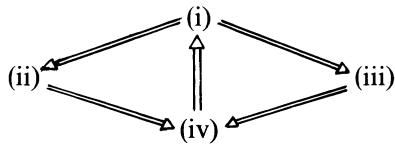
\includegraphics[keepaspectratio]{images/part002_fd83f186.jpg}}

若 \(u\) 是满射，则它是一个严格态射 (IV, 第 28 页, 定理 1)，于是对每个半范数 \(p \in \mathrm{S}(\mathrm{E})\)，存在半范数 \(q \in \mathrm{S}(\mathrm{F})\)，使得对所有 \(y \in \mathrm{F}\)（满足 \(q(y) \leqslant 1\) 者），存在 \(x \in \mathrm{E}\) 满足 \(p(x) \leqslant 1\) 且 \(u(x) = y\)。我们立即推出 (i) 蕴含 (ii) 与 (iii)。显然 (ii) 蕴含 (iv)。

为证 (iii) 蕴含 (iv)，设 \(p\) 与 \(q\) 如 (iii) 所述。设 \(y \in \mathbf{F}\)，由 (iii)，存在 \(x\)（属于 \(\mathbf{E}\)）使得 \(q(u(x) - y) = 0\)。若 \(f \in \mathbf{F}'\) 满足 \(|f \circ u| \leqslant p\)，则有 \(f(u(x) - y) = 0\)，于是

\[
\left| f (y) \right| = \left| f (u (x)) \right| \leqslant p (x)
\]

从而关系式 (1) 成立。

最后证明 (iv) 蕴含 (i)。设 \(p \in \mathrm{S}(\mathrm{E})\)，设 \(q\) 是诸函数 \(|f|\)（\(f \in \mathrm{F}'\) 取遍满足 \(|f \circ u| \leqslant p\) 者）的上包络。由 (iv)，\(q\) 在 \(\mathrm{F}\) 上有限，且显然是 \(\mathrm{F}\) 上的一个下半连续半范数；由于 \(\mathrm{F}\) 是桶型空间 (III, 第 25 页, 推论)，我们有 \(q \in \mathrm{S}(\mathrm{F})\)。设 \(\mathbf{B}_p\)（相应地，\(\mathbf{B}_q\)）表示所有 \(x \in \mathrm{E}\)（相应地，\(y \in \mathrm{F}\)）中满足 \(p(x) \leqslant 1\)（相应地，\(q(y) \leqslant 1\)）者所成的集。我们有 \(q \circ u \leqslant p\)，于是 \(u(\mathbf{B}_p) \subset \mathbf{B}_q\)。\(u(\mathbf{B}_p)\) 在 \(\mathrm{F}'\) 中的极集由这样的线性型 \(f \in \mathrm{F}'\) 组成：它们满足 \(|f \circ u| \leqslant p\)，从而 \(|f| \leqslant q\)；换句话说，我们得到 \(u(\mathbf{B}_p)^{\circ} \subset \mathbf{B}_q^{\circ}\)，最后，\(\overline{u(\mathbf{B}_p)} = \mathbf{B}_q\) 由双极定理 (II, 第 45 页, 推论 3) 得出。若 \(\mathrm{U}\) 是 \(\mathrm{E}\) 中 0 的一个邻域，则存在 \(p \in \mathrm{S}(\mathrm{E})\) 使得 \(\mathbf{B}_p \subset \mathbf{U}\)，于是 \(\overline{u(\mathbf{U})}\) 包含邻域 \(\mathbf{B}_q\)（即 \(\mathrm{F}\) 中 0 的邻域）。这就蕴含 \(u\) 是满射 (I, 第 17 页, 定理 1)。

推论. --- 设 E 与 F 是 Banach 空间。下列条件等价：

\begin{enumerate}
\def\labelenumi{(\roman{enumi})}
\item
  \(u\) 是满射。
\item
  存在实数 \(r > 0\)，使得 \(\| f \| \leqslant r\) . \(\| {}^t u(f) \|\) 对所有 \(f \in \mathbf{F}'\) 成立。
\item
  对所有 \(y \in F\)，我们有 \(\sup_{\substack{f\in \mathbf{F}^{\prime}\\ |f\circ u|\leqslant 1}} |f(y)| < +\infty\)。
\end{enumerate}

条件 (ii) 与 (iii) 实际上就是命题 4 的条件 (ii) 与 (iv) 在 Banach 空间情形下的重新表述。

\section{紧性判别法}

\subsection{一般注记}

设 A 是拓扑空间 E 的一个子集。为使 A 中点的一个序列 \((x_{n})_{n\in\mathbf{N}}\) 以 E 的一个点 x 为极限点，必须且只需下列条件成立 (GT, I, § 7, No.~3)：

\begin{enumerate}
\def\labelenumi{(\Alph{enumi})}
\tightlist
\item
  对每个整数 \(m \geqslant 0\) 以及每个邻域 \(\mathbf{U}\)（\(x\) 的一个邻域），存在一个整数 \(n \geqslant m\) 使得 \(x_{n} \in \mathbf{U}\)。
\end{enumerate}

形如 \((y_{k})_{k\in\mathbb{N}}\)（其中 \(y_{k}=x_{n_{k}}\)，\((n_{k})_{k\in\mathbb{N}}\) 是严格递增的正整数序列）的序列称为序列 \((x_{n})_{n\in\mathbb{N}}\) 的一个子序列。若序列 \((x_{n})_{n\in\mathbb{N}}\) 存在一个收敛到 x 的子序列，则 x 是 \((x_{n})\) 的一个极限点；反之，若 x 具有可数的基本邻域系，且 x 是序列 \((x_{n})\) 的极限点，则存在 \((x_{n})\) 的一个收敛到 x 的子序列。

根据 GT, IX, § 2, No.~9 的推论，我们断定，当 E 可度量化时，下列条件等价：

\begin{enumerate}
\def\labelenumi{\alph{enumi})}
\item
  集 A 在 E 中相对紧；
\item
  A 中点的每个无穷序列在 E 中有一个极限点；
\item
  从 A 中点的每个无穷序列，可以抽取出一个收敛到 E 中某点的序列。
\end{enumerate}

在本节中，我们将把这个判别法推广到某些不可度量化的拓扑向量空间。下面的命题使我们在许多情形下能把紧集的研究归结为弱紧集的研究。

命题 1. --- 设 E 是一个 Hausdorff 局部凸空间，A 是 E 的一个子集。设 \(E_{\sigma}\) 表示赋以弱化拓扑的空间 E。

\begin{enumerate}
\def\labelenumi{\alph{enumi})}
\item
  若 \(\mathbf{A}\) 中点的每个无穷序列在 \(\mathbf{E}\) 中有一个极限点，则 \(\mathbf{A}\) 在 \(\mathbf{E}\) 中预紧。
\item
  为使 A 在 E 中相对紧，必须且只需它在 E 中预紧且在 \(E_{\sigma}\) 中相对紧。
\end{enumerate}

我们用反证法证明 \(a)\)。若 \(A\) 不是预紧的，则由 GT, II, § 3, No.~7 的定理 3，可知存在一个对称凸邻域 \(V\)（\(E\) 中 0 的邻域），使得 \(A\) 不能被 \(V\) 的有限个平移所覆盖。

换句话说，若 \(x_{0}, x_{1}, \ldots, x_{n-1}\) 是 A 的点，则 \(A \not\subset \bigcup_{0 \leqslant i < n} (x_{i} + V)\)，于是存在 A 的一个点 \(x_{n}\) 使得 \(x_{n} - x_{i} \notin V\) 对 \(0 \leqslant i < n\) 成立。然后，对整数 n 用归纳法，可以构造 A 中点的一个无穷序列 \((x_{n})_{n \in \mathbb{N}}\)，使得 \(x_{n} - x_{m} \notin V\)（当 n \textgreater{} m 时）；由于 V 是对称的，我们还有 \(x_{m} - x_{n} \notin V\)（对 \(m \neq n\)），从而诸集 \(x_{n} + \frac{1}{2}V\) 两两不相交。对 E 中的每个点 x，至多存在一个整数 \(n \geqslant 0\) 使得 \(x_{n} \in x + \frac{1}{2}V\)，因而序列 \((x_{n})_{n \in \mathbb{N}}\) 没有任何极限点。这就证明了 a)。

现在假设 A 在 E 中预紧，并且包含在 \(E_{\sigma}\) 的一个紧子集 B 中。那么 B 在 \(E_{\sigma}\) 中完备，从而在 E 中也完备 (IV, 第 5 页, 注记 2)。我们有 \(\overline{A} \subset B\)，故 A 在 E 中相对紧。逆命题是显然的，b) 随之得证。

\subsection{连续函数集合的简单紧性}

在本节中，X 表示一个紧空间，\(\mathcal{C}_{s}(X)\) 表示 X 上以域 K（等于 R 或 C）为值的连续函数空间。空间 \(\mathcal{C}_{s}(X)\) 赋以 X 上的简单收敛拓扑。

命题 2. --- 设 D 是 X 的一个稠密子集，A 是空间 \(\mathcal{C}_{s}(X)\) 的一个子集。下列条件等价：

\begin{enumerate}
\def\labelenumi{(\roman{enumi})}
\item
  A 在 \(\mathcal{C}_s(\mathbf{X})\) 中相对紧。
\item
  从 \(\mathbf{A}\) 的元素的每个无穷序列，可以抽取一个在 \(\mathcal{C}_s(\mathbf{X})\) 中收敛的序列。
\item
  \(\mathbf{A}\) 的元素的每个无穷序列在 \(\mathcal{C}_s(\mathbf{X})\) 中有一个极限点。
\item
  设 \((f_n)_{n\in \mathbb{N}}\) 是属于 A 的函数序列，\((x_m)_{m\in \mathbb{N}}\) 是 D 的点的序列。若累次极限
\end{enumerate}

\[
\gamma = \lim _ {m \rightarrow \infty} \lim _ {n \rightarrow \infty} f _ {n} (x _ {m}), \quad \delta = \lim _ {n \rightarrow \infty} \lim _ {m \rightarrow \infty} f _ {n} (x _ {m})
\]

存在，则它们相等。此外，我们有 \(\sup_{f\in \mathbf{A}}|f(x)| < +\infty\)（对所有 \(x\in \mathbf{X}\)）。

\begin{enumerate}
\def\labelenumi{(\roman{enumi})}
\tightlist
\item
  \(\Rightarrow\) (ii)：设 \(\overline{\mathbf{A}}\) 是 \(\mathbf{A}\) 在 \(\mathcal{C}_s(\mathbf{X})\) 中的闭包。假设 \(\mathbf{A}\) 是紧的，并考虑函数序列 \(f_n \in \mathbf{A}\)（\(n \in \mathbf{N}\)）。设 \(\phi\) 是连续映射 \(x \mapsto (f_n(x))_{n \in \mathbf{N}}\)（从 \(\mathbf{X}\) 到可度量化空间 \(\mathbf{K}^{\mathbf{N}}\) 中的映射）。像 \(\mathbf{X}'\)（即 \(\mathbf{X}\) 在 \(\phi\) 下的像）是一个紧可度量化空间，因为 \(\mathbf{X}\) 是紧的。设 \(\mathbf{E}\) 是 \(\mathcal{C}_s(\mathbf{X})\) 的闭子空间，由满足下列条件的连续函数 \(f\)（定义在 \(\mathbf{X}\) 上）组成：关系 \(\phi(x) = \phi(y)\) 蕴含 \(f(x) = f(y)\)（\(x, y\) 是 \(\mathbf{X}\) 中任意一对点）。根据 GT, I, § 9, No.~4 的推论 2 与 GT, I, § 5, No.~2 的命题 3，映射 \(f' \mapsto f' \circ \phi\) 是一个同胚 \(\phi^*\)（从 \(\mathcal{C}_s(\mathbf{X}')\) 到 E 上）。因此，集 \(\mathbf{A}' = (\phi^*)^{-1}(\overline{\mathbf{A}})\) 在 \(\mathcal{C}_s(\mathbf{X}')\) 中是紧的，并且显然存在元素 \(f_n'\)（属于 \(\mathbf{A}'\)）使得 \(\phi^*(f_n') = f_n' \circ \phi\) 等于 \(f_n\)。
\end{enumerate}

由于 \(X'\) 是一个紧可度量化空间，存在一个可数稠密子集 \(D'\)（在 \(X'\) 中）(GT, IX, §2, No.~8, 命题 12 与 §2, No.~9, 命题 16)。设 \(T_{1}\)（相应地，\(T_{2}\)）是 \(A'\) 上由 \(D'\)（相应地，\(X'\)）上的简单收敛拓扑诱导的拓扑。那么 \(T_{1}\) 可度量化，\(T_{2}\) 紧且比 \(T_{1}\) 细，因而 \(T_{1}\) 与 \(T_{2}\) 一致；换句话说，\(A'\) 是 \(\mathcal{C}_{s}(X')\) 的一个紧可度量化子空间。从而，存在一个序列 \((f_{n_k}^{\prime})\)（从 \((f_n^{\prime})\) 中抽取），它收敛到某个元素 \(f^{\prime}\)（属于 \(\mathcal{C}_s(\mathbf{X}')\)）。因此，序列 \((f_{n_k})\) 收敛到 \(f = f' \circ \phi\)（在 \(\mathcal{C}_s(\mathbf{X})\) 中）。

\begin{enumerate}
\def\labelenumi{(\roman{enumi})}
\setcounter{enumi}{1}
\item
  \(\Rightarrow\) (iii)：这是显然的。
\item
  \(\Rightarrow\) (iv)：假设 A 的元素的每个无穷序列在 \(\mathcal{C}_s(\mathbf{X})\) 中有一个极限点。设 \(x \in \mathbf{X}\)。映射 \(\phi_x: f \mapsto f(x)\)（从 A 到 K 中的映射）是连续的。于是，\(\phi_x(\mathbf{A})\) 中的每个无穷序列有一个极限点；由于域 K（等于 R 或 C）可度量化，集 \(\phi_x(\mathbf{A})\) 在 K 中相对紧，从而有界。换句话说，我们有 \(\sup_{f \in \mathbf{A}} |f(x)| < \infty\)。
\end{enumerate}

设 \(f_n, x_m, \gamma\) 与 \(\delta\) 如 (iv) 所述。设 \(f\) 是序列 \((f_n)\) 在 \(\mathcal{C}_s(\mathbf{X})\) 中的一个极限点，设 \(x\) 是序列 \((x_m)\) 在紧空间 \(\mathbf{X}\) 中的一个极限点。对每个 \(m\)，映射 \(h \mapsto h(x_m)\)（从 \(\mathcal{C}_s(\mathbf{X})\) 到 \(\mathbf{K}\) 中）是连续的。根据假设，我们有 \(f(x_m) = \lim_{n \to \infty} f_n(x_m)\)，从而 \(\gamma = \lim_{m \to \infty} f(x_m)\)；由于 \(f: \mathbf{X} \to \mathbf{K}\) 连续且 \(x\) 是序列 \((x_m)\) 的一个极限点，我们得到 \(\gamma = f(x)\)。用类似的方式，我们证明等式 \(\delta = f(x)\)，从而 \(\gamma = \delta\)。

\begin{enumerate}
\def\labelenumi{(\roman{enumi})}
\setcounter{enumi}{3}
\tightlist
\item
  \(\Rightarrow\) (i)：假设数 \(f(x)\)（当 \(f\) 取遍 \(\mathbf{A}\) 时）所成的集在 \(\mathbf{K}\) 中有界（对所有 \(x\in \mathbf{X}\)）。这等价于假设闭包 \(\overline{\mathbf{A}}\)（即 \(\mathbf{A}\) 在乘积空间 \(\mathbf{K}^{\mathbf{X}}\) 中的闭包）是紧的 (GT, I, § 9, No.~5)。假设 \(\mathbf{A}\) 在 \(\mathcal{C}_s(\mathbf{X})\) 中不是相对紧的。这就意味着存在一个函数 \(u\in \overline{\mathbf{A}}\) 和一个点 \(a\in \mathbf{X}\)，使得 \(u\) 在 \(a\) 处不连续。于是存在实数 \(\varepsilon >0\)，使得在每个邻域 \(\mathrm{U}\)（\(a\) 的邻域）中，存在一点 \(x\) 满足 \(|u(x) - u(a)|\geqslant \varepsilon\)。
\end{enumerate}

我们将用归纳法构造点的序列 \((x_{n})_{n\in \mathbf{N}}\)（点取自 \(\mathbf{D}\)）与元素的序列 \((f_n)_{n\in \mathbf{N}}\)（元素取自 \(\mathbf{A}\)），使它们满足下列关系：

\[
\left| u (x _ {m}) - u (a) \right| \geqslant \varepsilon \quad \text { for } \quad m \geqslant 1;\tag{$(1)_{m}$}
\]

\[
\left| u (x _ {i}) - f _ {m} (x _ {i}) \right| \leqslant \frac {1}{m + 1} \text { for } 0 \leqslant i \leqslant m - 1;\tag{$(2)_{m}$}
\]

\[
\left| f _ {m} (x _ {i}) - f _ {m} (a) \right| \leqslant \frac {1}{i + 1} \quad \text { for } \quad 0 \leqslant m \leqslant i.\tag{$(3)_{m,i}$}
\]

我们取 \(x_0 = a\)，其中 \(f_0\) 是 A 中任意取的（集 A 非空，否则它在 \(\mathcal{C}_s(\mathbf{X})\) 中将相对紧）。设 \(n \geqslant 1\)，且 \(x_0, x_1, \ldots, x_{n-1}, f_0, f_1, \ldots, f_{n-1}\) 满足关系式 \((1)_m, (2)_m\)（对 \(1 \leqslant m < n\)）与 \((3)_{m,i}\)（对 \(0 \leqslant m \leqslant i < n\)）。由于 \(u\) 属于 \(\overline{\mathbf{A}}\)，存在 \(f_n \in \mathbf{A}\) 满足 \((2)_n\)。设 \(V_n\) 是所有 \(x \in X\) 中满足 \(|f_m(x) - f_m(a)| \leqslant \frac{1}{n+1}\)（对 \(0 \leqslant m \leqslant n\)）者所成的集。由于 \(f_n\) 连续，\(V_n\) 是 \(a\) 的一个邻域；选取一点 \(x_n\)（在 \(D \cap V_n\) 中）使得 \(|u(x_n) - u(a)| \geqslant \varepsilon\)，于是 \((1)_n\) 与 \((3)_{m,n}\) 得到满足。因此，构造可以继续进行。

由于 \(u(\mathbf{X})\) 是 \(\mathbf{K}\) 的一个紧子集，存在一个序列 \((y_k)\)（从 \((x_m)\) 中抽取），使得极限 \(\gamma = \lim_{k\to \infty}u(y_k)\) 存在。由 (2) \(_m\)，我们有 \(u(x_i) = \lim_{n\to \infty}f_n(x_i)\)（对所有 \(i\in \mathbf{N}\)），从而

\[
\gamma = \lim _ {k \rightarrow \infty} \lim _ {n \rightarrow \infty} f _ {n} (y _ {k}).\tag{4}
\]

另一方面，我们有 \(f_{n}(a) = \lim_{i\to \infty}f_{n}(x_{i})\)（由 (3) \(_{m,i}\)），从而 \(f_{n}(a) = \lim_{k\to \infty}f_{n}(y_{k})\)。由于 \(x_0 = a\)，由 (2) \(_{m}\) 推出 \(\lim_{n\to \infty}f_n(a) = u(a)\)。于是，

\[
u (a) = \lim _ {n \rightarrow \infty} \lim _ {k \rightarrow \infty} f _ {n} (y _ {k}).\tag{5}
\]

最后，由 \((1)_{m}\) 得到 \(|\gamma - u(a)| \geqslant \varepsilon\)，于是 \(\gamma \neq u(a)\)。这与断言 (iv) 矛盾；这样我们就证明了 (iv) 蕴含 (i)。

\subsection{Eberlein 定理与 Šmulian 定理}

定理 1 (Eberlein). --- 设 E 是一个 Hausdorff 且拟完备的局部凸空间，T 是 E 上与 E 和 E′ 之间的对偶相容的一个拓扑，A 是 E 的一个子集。为使 A 对于 T 相对紧，必须且只需 A 中点的每个无穷序列对于 T 在 E 中有一个极限点。

所述条件显然是必要的。

现在假设 A 中点的每个无穷序列对于 T 有一个极限点，从而对于较粗的拓扑 \(\sigma(\mathrm{E}, \mathrm{E}')\) 也有一个极限点。那么 A 对于 T 预紧 (IV, 第 32 页, 命题 1)；为使 A 对于 T 相对紧，必须且只需它对于 \(\sigma(\mathrm{E}, \mathrm{E}')\) 相对紧（出处同上）。因此只需对 T 是弱化拓扑 \(\sigma(\mathrm{E}, \mathrm{E}')\) 的情形证明本定理。

设 \(\hat{\mathrm{E}}\) 是 E 的完备化，我们照例把它与代数对偶 \(\mathrm{E}^{\prime *}\)（\(\mathrm{E}'\) 的代数对偶）的一个子空间视为同一 (III, 第 21 页, 定理 2)。设 \(\mathrm{E}_{\sigma}\)、\(\hat{\mathrm{E}}_{\sigma}\) 与 \(\mathrm{E}_{\sigma}^{\prime *}\) 分别表示空间 E、\(\hat{\mathrm{E}}\) 与 \(\mathrm{E}^{\prime *}\)，各赋以拓扑 \(\sigma (\mathrm{E},\mathrm{E}')\)、\(\sigma (\hat{\mathrm{E}},\mathrm{E}')\) 与 \(\sigma (\mathrm{E}^{\prime *},\mathrm{E}^{\prime})\)。

设 \((x_{i}^{\prime})_{i\in\mathbb{I}}\) 是向量空间 \(E^{\prime}\) 在域 K 上的一个基。映射 \(f\mapsto(f(x_{i}^{\prime}))_{i\in\mathbb{I}}\) 是一个同胚 \(\phi\)（从 \(E_{\sigma}^{\prime*}\) 到 \(K^{I}\) 上）；对每个 \(i\in I\)，A 在映射 \(x_{i}^{\prime}\)（从 E 到 K 中的映射）下的像是相对紧的：因为 K 可度量化，且 \(x_{i}^{\prime}(A)\) 的元素的每个无穷序列有一个极限点。由此推出 \(\phi(A)\) 在 \(K^{I}\) 中相对紧，从而闭包 \(\overline{A}\)（A 在 \(E_{\sigma}^{\prime*}\) 中的闭包）是紧的。

其次我们证明 \(\overline{A}\) 包含在 \(\hat{E}\) 中。设 H 是 \(E'\) 的一个等度连续子集；设 X 是它对于 \(\sigma(E', E)\) 的闭包；X 是紧的 (III, 第 17 页, 推论 2)。对每个 \(x \in E'^{*}\)，设 \(\phi_{x}\) 是 \(x' \mapsto \langle x, x' \rangle\) 在 X 上的限制；设 \(\tilde{A} \subset \mathcal{C}_{s}(X)\) 是当 x 取遍 A 时函数 \(\phi_{x}\) 所成的集。鉴于关于 A 的假设，\(\tilde{A}\) 的元素的每个无穷序列在 \(\mathcal{C}_{s}(X)\) 中有一个极限点；由命题 2 (IV, 第 33 页)，集 \(\tilde{A}\) 因而在 \(\mathcal{C}_{s}(X)\) 中相对紧。由此推出，对每个 \(a \in \overline{A}\)，X 上的函数 \(\phi_{a}\) 是连续的。包含关系 \(\overline{A} \subset \hat{E}\) 于是由 III, 第 21 页 的定理 2 得出。

现在我们证明 \(\overline{\mathbf{A}}\) 包含在 E 中。由于 A 在 \(\mathrm{E}_{\sigma}\) 中预紧 (IV, 第 32 页, 命题 1)，它在 \(\mathrm{E}_{\sigma}\) 中有界 (III, 第 3 页, 命题 2)，从而在 E 中也有界 (IV, 第 1 页, 命题 1)。设 C 是 A 在 E 中的闭均衡凸包。那么 C 有界（因 A 有界），从而完备（因 E 拟完备）。换句话说，C 是 \(\hat{\mathrm{E}}\) 的一个凸闭子集，因而也是 \(\hat{\mathrm{E}}_{\sigma}\) 的凸闭子集 (IV, 第 1 页, 命题 1)。由于 \(\mathbf{A} \subset \mathbf{C}\) 且 \(\hat{\mathrm{E}}_{\sigma}\) 的拓扑由 \(\mathrm{E}_{\sigma}^{\prime *}\) 的拓扑诱导，我们有 \(\overline{\mathbf{A}} \subset \mathbf{C}\)，从而 \(\overline{\mathbf{A}} \subset \mathbf{E}\)。

由于 \(E_{\sigma}\) 的拓扑由 \(E_{\sigma}^{\prime*}\) 的拓扑诱导，子集 \(\overline{A}\)（\(E_{\sigma}\) 的子集）是紧的，定理 1 随之得证。

定理 2 (Šmulian). --- 设 E 是一个 Fréchet 空间，A 是 E 的一个子集。设 \(E_{\sigma}\) 表示赋以弱化拓扑的空间 E。下列条件等价：

\begin{enumerate}
\def\labelenumi{(\roman{enumi})}
\item
  A 在 \(\mathrm{E}_{\sigma}\) 中相对紧；
\item
  A 中点的每个无穷序列在 \(\mathrm{E}_{\sigma}\) 中有一个极限点；
\item
  从 \(\mathbf{A}\) 中点的每个无穷序列，可以抽取一个在 \(\mathrm{E}_{\sigma}\) 中收敛的序列。
\end{enumerate}

(i) 与 (ii) 的等价性由 Eberlein 定理得出，且 (iii) 显然蕴含 (ii)。

我们来证明 (i) 蕴含 (iii)。假设 A 在 \(E_{\sigma}\) 中的闭包 B 是紧的，且 \((x_{n})_{n\in\mathbf{N}}\) 是 A 的点的一个序列。设 F 是 E 中包含诸 \(x_{n}\) 的最小闭向量子空间，它是一个满足第一可数公理的 Fréchet 空间。由于 F 在 \(E_{\sigma}\) 中闭，且 F 上的拓扑 \(\sigma(\mathrm{F},\mathrm{F}')\) 由 \(\sigma(\mathrm{E},\mathrm{E}')\) 诱导，集 \(B\cap F\) 对于 \(\sigma(\mathrm{F},\mathrm{F}')\) 是紧的。根据 IV, 第 32 页 的注记，从 \((x_{n})_{n\in\mathbf{N}}\) 中抽取一个对于 \(\sigma(\mathrm{E},\mathrm{E}')\)（或者等价地，对于 \(\sigma(\mathrm{F},\mathrm{F}')\)）收敛的序列，其存在性是下述引理的推论：

引理 1. --- 设 F 是一个满足第一可数公理的 Fréchet 空间。F 的每个对于拓扑 T（由 \(\sigma(\mathrm{F},\mathrm{F}')\) 诱导）紧的子集 C 对于该拓扑可度量化。

由于 \(F'\) 上的预紧收敛拓扑比拓扑 \(\sigma(F', F)\) 细，在 \(F_{s}'\) 中存在一个处处稠密的可数子集 (III, 第 18 页, 推论 1)。于是集 C 可以与 \(K^{D}\) 的一个子集视为同一，且 \(K^{D}\) 的拓扑（它可度量化 (GT, IX, § 2, No.~8)）在 C 上诱导的拓扑比由 \(\sigma(F, F')\) 诱导的拓扑粗，而 C 对于后者是紧的。因此这两个拓扑相同 (GT, I, § 9, No.~4, 推论 3)。

Šmulian 定理可以推广到 E 是一列 Fréchet 空间的严格归纳极限的情形 (IV, 第 67 页, 习题 2)。

\subsection{* 有界连续函数空间的情形}

对每个拓扑空间 X，设 \(\mathcal{C}^{b}(X)\) 表示从 X 到 K 中的所有连续且有界的映射所成的 Banach 空间，赋以由下式定义的范数

\[
\| f \| = \sup _ {x \in X} | f (x) |\tag{6}
\]

(GT, X, § 3, No.~2)。当 X 紧时，X 上的每个连续函数都有界 (GT, IV, § 6, No.~1)，我们把 \(\mathcal{C}(X)\) 记作 \(\mathcal{C}^b(X)\)。

在本节及下一节中，我们将用到下面的引理，它是 Lebesgue 定理 (INT, IV, 第 2 版, § 4, No.~3, 定理 2) 的一个特例，这里用到把 \(\mathcal{C}(\mathrm{X})'\) 的元素解释为 X 上的测度。

引理 2. --- 设 X 是一个紧空间。若序列 \((f_n)_{n\in \mathbf{N}}\) 在 \(\mathcal{C}(\mathbf{X})\) 中有界且在 X 上简单收敛到连续函数 \(f\)，则 \(\mu(f) = \lim_{n\to \infty}\mu(f_n)\) 对每个 \(\mu\)（属于 \(\mathcal{C}(\mathbf{X})'\)）成立。

命题 3. --- 设 X 是一个紧空间，A 是 \(\mathcal{C}(\mathrm{X})\) 的一个有界子集。为使 A 对于简单收敛拓扑相对紧，必须且只需它对于 \(\sigma(\mathcal{C}(\mathrm{X}), \mathcal{C}(\mathrm{X})')\) 相对紧。

简单收敛拓扑是 Hausdorff 的且比 \(\sigma(\mathcal{C}(X), \mathcal{C}(X)')\) 粗，故所述条件是充分的 (GT, I, § 9, No.~4, 推论 3)。

现在假设 A 对于简单收敛拓扑相对紧。设 \((f_{n})_{n\in\mathbf{N}}\) 是 A 的元素的一个序列。由命题 2 (IV, 第 33 页)，存在一个序列 \((f_{n_{k}})\)（从 \((f_{n})\) 中抽取），它简单收敛到一个连续函数 f。由引理 2，有界序列 \((f_{n_{k}})\) 对于 \(\sigma(\mathcal{C}(\mathrm{X}),\mathcal{C}(\mathrm{X})')\) 趋于 f。于是 Šmulian 定理 (IV, 第 36 页, 定理 2) 表明 A 对于 \(\sigma(\mathcal{C}(\mathrm{X}),\mathcal{C}(\mathrm{X})')\) 相对紧。

推论. --- 设 S 是一个拓扑空间，A 是 \(\mathcal{C}^{b}(S)\) 的一个有界子集。下列条件等价：

\begin{enumerate}
\def\labelenumi{(\roman{enumi})}
\item
  A 对于 \(\sigma(\mathcal{C}^b(\mathbf{S}),\mathcal{C}^b(\mathbf{S})')\) 相对紧；
\item
  若 \((f_n)_{n\in \mathbb{N}}\) 是 \(\mathbf{A}\) 的元素的序列，\((x_m)_{m\in \mathbb{N}}\) 是 \(\mathbf{S}\) 的点的序列，且累次极限
\end{enumerate}

\[
\gamma = \lim _ {m \rightarrow \infty} \lim _ {n \rightarrow \infty} f _ {n} (x _ {m}), \quad \delta = \lim _ {n \rightarrow \infty} \lim _ {m \rightarrow \infty} f _ {n} (x _ {m})
\]

存在，则 \(\gamma = \delta\)。

设 X 是 S 的 Stone-Čech 紧化 (GT, IX, § 1, No.~6)，\(\alpha\) 是从 S 到 X 中的典范映射。令 \(D = \alpha(S)\)。映射 \(\phi: f \mapsto f \circ \alpha\) 是从赋范空间 \(\mathcal{C}(X)\) 到赋范空间 \(\mathcal{C}^b(S)\) 上的一个同构；令 \(\tilde{A} = \phi^{-1}(A)\)。由于 X 紧且 D 在 X 中稠密，命题 2 (IV, 第 33 页) 表明条件 (ii) 等价于 \(\tilde{A}\) 对于简单收敛拓扑的紧性。(i) 与 (ii) 的等价性于是由命题 3 得出。*

\subsection{* 弱紧集的凸包}

定理 3 (Krein). --- 设 E 是一个 Hausdorff 且拟完备的局部凸空间，T 是 E 上与 E 和 E′ 之间的对偶相容的一个拓扑。设 A 是 E 的一个对于 T 紧的子集。那么 A 的闭均衡凸包 C 对于 T 是紧的。

我们先作若干约化。

\begin{enumerate}
\def\labelenumi{\Alph{enumi})}
\item
  集 C 对于 \(\mathcal{T}\) 预紧 (II, 第 25 页, 命题 3)，且 A 对于 \(\sigma(\mathrm{E}, \mathrm{E}')\) 紧。根据命题 1 (IV, 第 32 页)，只需证明 C 对于 \(\sigma(\mathrm{E}, \mathrm{E}')\) 紧，于是我们已约化到 \(\mathcal{T} = \sigma(\mathrm{E}, \mathrm{E}')\) 的情形。
\item
  由于 C 对于 \(\sigma(\mathrm{E}, \mathrm{E}')\) 预紧且闭，它对于 E 的初始拓扑有界且闭 (III, 第 3 页, 命题 2 与 IV, 第 1 页, 命题 1)；从而由于 E 拟完备，它是完备的。换句话说，C 是 A 在 E 的完备化 \(\hat{\mathbf{E}}\) 中的闭均衡凸包。由于拓扑 \(\sigma (\hat{\mathbf{E}},\mathrm{E}^{\prime})\) 在 E 上诱导 \(\sigma (\mathrm{E},\mathrm{E}^{\prime})\)，我们已约化到 E 完备的情形。
\item
  设 \(\Gamma\) 是 A 的均衡凸包。那么 C 是 \(\Gamma\) 对于 \(\sigma(E, E')\) 的闭包。由 Eberlein 定理 (IV, 第 35 页, 定理 1)，只需证明点的每个序列 \((x_n)_{n \in \mathbf{N}}\)（点取自 \(\Gamma\)）在 E 中对于 \(\sigma(E, E')\) 有一个极限点。但 \(x_n\) 属于 A 的有限子集 \(\mathbf{B}_n\) 的均衡凸包。设 F 是由可数集 \(\mathbf{B} = \bigcup_{n} \mathbf{B}_n\) 生成的 E 的闭向量子空间。那么 F 完备，F 上的拓扑 \(\sigma(F, F')\) 由 \(\sigma(E, E')\) 诱导，且我们有 \(x_n \in F\)（对所有 \(n \in \mathbf{N}\)）。因而只需证明 \((x_n)_{n \in \mathbf{N}}\) 对于 \(\sigma(F, F')\) 有一个极限点，这就给出了到 E 中存在可数稠密集的情形的约化。
\end{enumerate}

设 A 赋以由 \(\sigma(E, E')\) 诱导的拓扑，这使它成为一个紧空间。我们定义一个线性映射 \(u: E' \to \mathcal{C}(A)\) 如下

\[
u (x ^ {\prime}) (a) = \langle a, x ^ {\prime} \rangle \quad (a \in \mathrm{A}, x ^ {\prime} \in \mathrm{E} ^ {\prime}).\tag{7}
\]

设 \((x_{n}^{\prime})_{n\in\mathbb{N}}\) 是 E′ 中的一个等度连续序列，它对于 \(\sigma(\mathrm{E}^{\prime},\mathrm{E})\) 收敛到 0。那么函数序列 \(u(x_{n}^{\prime})\) 在 \(\mathcal{C}(\mathrm{A})\) 中有界且简单收敛到 0。对每个 \(\mu\in\mathcal{C}(\mathrm{A})^{\prime}\)，由引理 2 (IV, 第 37 页)，我们有 \(\lim_{n\to\infty}\mu(u(x_{n}^{\prime}))=0\)。根据 III, 第 21 页 的注记中给出的判别法，E′ 上的线性型 \(\mu\circ u\) 于是对于 \(\sigma(\mathrm{E}^{\prime},\mathrm{E})\) 连续（对每个 \(\mu\in\mathcal{C}(\mathrm{A})^{\prime}\)）。因此存在一个线性映射 \(v:\mathcal{C}(\mathrm{A})^{\prime}\to\mathrm{E}\) 满足关系式

\[
\langle u (x ^ {\prime}), \mu \rangle = \langle v (\mu), x ^ {\prime} \rangle \quad \left(x ^ {\prime} \in \mathrm{E} ^ {\prime}, \mu \in \mathcal {C} (\mathrm{A}) ^ {\prime}\right).\tag{8}
\]

显然，\(v\) 是连续的，若 \(\mathcal{C}(\mathbf{A})'\) 赋以拓扑 \(\sigma(\mathcal{C}(\mathbf{A})', \mathcal{C}(\mathbf{A}))\)，而 \(E\) 赋以拓扑 \(\sigma(E, E')\)。

Banach 空间 \(\mathcal{C}(\mathrm{A})\) 的（闭）单位球 B 对于拓扑 \(\sigma(\mathcal{C}(\mathrm{A})', \mathcal{C}(\mathrm{A}))\) 是紧的 (III, 第 17 页, 推论 3)。于是，\(v(\mathrm{B})\) 是 E 的一个对于 \(\sigma(\mathrm{E}, \mathrm{E}')\) 的凸均衡紧子集。对每个 \(a \in A\)，连续线性型 \(\varepsilon_a : f \mapsto f(a)\)（\(\mathcal{C}(\mathrm{A})\) 上的连续线性型）属于 B，且由公式 (7) 与 (8) 我们有 \(v(\varepsilon_a) = a\)。因此，\(A \subset v(\mathrm{B})\)，从而 \(C \subset v(\mathrm{B})\)。这就证明了 C 对于 \(\sigma(\mathrm{E}, \mathrm{E}')\) 是紧的。

证毕。

\chapterappendix{仿射变换群的不动点}

\subsection{可解群的情形}

设 \(\mathbf{E}\) 是一个实向量空间，\(\mathbf{K}\) 是 \(\mathbf{E}\) 的一个凸子集。一个映射 \(u: \mathbf{K} \to \mathbf{K}\)，若对 \(x, y\)（属于 \(\mathbf{K}\)）以及对每个实数 \(t\)（属于 \([0, 1]\)），我们有

\[
u (t x + (1 - t) y) = t u (x) + (1 - t) u (y)\tag{1}
\]

就称为一个仿射变换。由关系式 (1) 我们推出

\[
u \left(\sum_ {i \in \mathrm{I}} t _ {i} x _ {i}\right) = \sum_ {i \in \mathrm{I}} t _ {i} u \left(x _ {i}\right)\tag{2}
\]

对每个有限集 I、K 中的点 \(x_{i}\) 以及正实数 \(t_i\)（满足 \(\sum_{i\in I}t_i = 1\)）成立。

设 u 与 v 是 K 上的两个仿射变换，则映射 \(u \circ v\) 是 K 上的一个仿射变换。若 \(v: E \to E\) 是一个满足 \(v(\mathbf{K}) \subset \mathbf{K}\) 的线性映射，则在 K 上与 v 相同的映射 \(u: K \to K\) 是一个仿射变换。

定理 1 (Markoff-Kakutani). --- 设 E 是域 R 上的一个 Hausdorff 局部凸向量空间，K 是 E 的一个非空紧凸子集。设 \(\Gamma\) 是 K 上的一组两两可交换的连续仿射变换。那么存在 K 中的一点 a，使得 \(u(a) = a\) 对所有 \(u \in \Gamma\) 成立。

对每个 \(u \in \Gamma\)，设 \(\mathbf{K}_u\) 是所有 \(x \in \mathbf{K}\) 中满足 \(u(x) = x\) 者所成的集。我们将证明 \(\mathbf{K}_u\) 非空。设 \(x\) 是 \(\mathbf{K}\) 的一个点；对每个整数 \(n \geqslant 1\)，设 \(x_n\) 是元素 \(\frac{1}{n} \sum_{i=0}^{n-1} u^i(x)\)（\(\mathbf{E}\) 中的元素）。由于 \(\mathbf{K}\) 凸且在 \(u\) 下稳定，诸点 \(x_n\) 属于 \(\mathbf{K}\)，且由于 \(\mathbf{K}\) 紧，存在一个极限点 \(a\)（序列 \((x_n)_{n \geqslant 1}\) 的极限点）。映射 \(y \mapsto u(y) - y\)（从 \(\mathbf{K}\) 到 \(\mathbf{E}\) 中的映射）是连续的，因而 \(u(a) - a\) 是序列 \((u(x_n) - x_n)_{n \geqslant 1}\) 的一个极限点。但我们有 \(u(x_n) - x_n = \frac{1}{n} (u^n(x) - x)\)。

由于 K 紧，从而有界 (III, 第 3 页, 命题 2)，序列 \((u^n(x) - x)_{n\geqslant 1}\) 有界；于是序列 \(\left(\frac{1}{n} (u^n (x) - x)\right)_{n\geqslant 1}\) 趋于 0 (III, 第 4 页, 命题 3)，且由于 E 是 Hausdorff 的，我们有 \(u(a) - a = 0\)。因此 \(a\in \mathbf{K}_u\)。

诸集 \(\mathbf{K}_u\) 中的每一个都是紧空间 \(\mathbf{K}\) 的闭凸子集，我们将证明交 \(\bigcap_{u\in \Gamma}\mathbf{K}_u\) 非空。为此只需

证明：对 \(n \geqslant 1\) 以及 \(u_{1}, \ldots, u_{n}\)（属于 \(\Gamma\)），集 \(K_{u_{1}} \cap \ldots \cap K_{u_{n}}\) 非空。n = 1 的情形已经考虑过，我们对 n 用归纳法论证。设 \(n \geqslant 2\)，并令 \(L = K_{u_{1}} \cap \ldots \cap K_{u_{n-1}}\)。由归纳假设，L 是 E 的一个非空紧凸子集。由于 \(u_{n}\) 与 \(u_{1}, \ldots, u_{n-1}\) 交换，我们有 \(u_{n}(L) \subset L\)。把证明的第一部分应用于 \(u_{n}\) 在 L 上诱导的仿射变换，我们断定存在 L 中的一点 a 使得 \(u_{n}(a) = a\)；于是 a 属于 \(K_{u_{1}} \cap \ldots \cap K_{u_{n}}\)，从而该集非空。

推论. --- 设 G 是 K 上连续仿射变换的一个可解群。那么存在 K 中的一点，它在 G 下不变。

根据可解群的定义 (A, I, § 6, No.~4)，存在一个有限递降序列 \((\mathbf{G}_i)_{0\leqslant i\leqslant n}\)（由 \(\mathbf{G}\) 的互不相同的子群组成），使得 \(\mathbf{G}_0 = \mathbf{G}\)，\(\mathbf{G}_n = \{e\}\)，且群 \(\mathbf{G}_{i - 1} / \mathbf{G}_i\) 对 \(1\leqslant i\leqslant n\) 是交换的。设 \(\mathbf{K}_i\) 表示 \(\mathbf{G}_i\) 在 \(\mathbf{K}\) 中的不动点集。那么 \(\mathbf{K}_n = \mathbf{K}\)。此外，对 \(1\leqslant i\leqslant n\)，\(\mathbf{G}_i\) 的每个元素在 \(\mathbf{K}_i\) 上诱导恒等变换；这样，我们就得到交换群 \(\mathbf{G}_{i - 1} / \mathbf{G}_i\) 在 \(\mathbf{K}\) 上的一个作用（若 \(\mathbf{K}_i\) 非空）；由定理 1 可知，不动点集 \(\mathbf{K}_{i - 1}\)（\(\mathbf{G}_{i - 1} / \mathbf{G}_i\) 在 \(\mathbf{K}_i\) 中的不动点集）非空。对 \(i\) 用递降归纳法，我们断定 \(\mathbf{K}_0\) 非空，推论得证。

\subsection{不变均值}

设 X 是一个拓扑空间。设 \(\mathcal{B}(\mathrm{X};\mathbf{R})\) 表示由 X 到 R 中的连续有界映射所成的实向量空间。赋以范数 \(\| f\| = \sup_{x\in \mathbf{X}}|f(x)|\)，它是一个 Banach 空间 (GT, X, § 3, No.~1)；它也是一个序向量空间，其中关系 \(f\geqslant g\) 表示 \(\ll f(x)\geqslant g(x) \text{ 对所有 } x\in \mathbf{X}\gg\)。

定义 1. --- 一个正线性型 \(\mu\)（空间 \(\mathcal{B}(\mathbf{X};\mathbf{R})\) 上的，其中 \(\mathbf{X}\) 是一个拓扑空间），若满足 \(\|\mu\| = 1\)，就称为 \(\mathbf{X}\) 上的一个均值。

* 当 X 紧时，X 上的一个均值是 X 上的一个正测度，且满足 \(\mu(X)=1\)。*

引理 1. --- X 上的均值所成的集 K 是 Banach 空间 \(E = \mathcal{B}(X; \mathbf{R})\) 的对偶的单位球的这样一个子集：其元素是线性型 \(\mu\)（满足 \(\mu(1)=1\) 者）。它是 \(E'\) 的一个对于 \(\sigma(E', E)\) 凸且紧的子集。

设 \(\mu\) 是 \(E\) 上的一个线性型，满足 \(\mu(1) = 1\)。对每个函数 \(f \in E\)，我们定义函数 \(f' \in E\) 为 \(f'(x) = \| f \| - f(x) (x \in X)\)。首先假设 \(\mu\) 是一个均值；对每个 \(f \in E\)，我们有 \(f' \geqslant 0\)，从而 \(\mu(f') \geqslant 0\)，即 \(\mu(f) \leqslant \| f \|\)；因此 \(\|\mu\| \leqslant 1\)。

反之，假设 \(\mu\) 属于 \(E'\)，且 \(\| \mu \| \leqslant 1\)；对每个正函数 \(f \in E\)，我们有 \(\mu(f') \leqslant \| f'\|\)，从而

\[
\| f \| - \mu (f) = \mu \left(f ^ {\prime}\right) \leqslant \| f ^ {\prime} \| \leqslant \| f \|,
\]

最后 \(\mu(f) \geqslant 0\)；于是，\(\mu\) 是一个均值。

显然 K 是凸的；它对于 \(\sigma(\mathrm{E}^{\prime},\mathrm{E})\) 的紧性由 III, 第 17 页 的推论 3 得出。

证毕。

设 \(\Gamma\) 是 X 到 X 中的两两交换的连续映射所成的一个集。设 \(\gamma \in \Gamma\)。对每个函数 \(f \in \mathbf{E}\)，我们有 \(f \circ \gamma \in \mathbf{E}\)；于是我们可以在 X 上的均值所成的集 K 上定义一个仿射变换 \(u_{\gamma}\)，如下

\[
u _ {\gamma} \mu (f) = \mu (f \circ \gamma) (\mu \in \mathrm{K}, f \in \mathrm{E}).
\]

若 K 赋以由 \(\sigma(\mathrm{E}^{\prime},\mathrm{E})\) 诱导的拓扑，则映射 \(u_{\gamma}\) 是连续的。若 \(\gamma\) 是一个同胚，\(u_{\gamma}\mu\) 可由 \(\mu\) 通过结构转移得到。最后，我们有 \(u_{\gamma}u_{\gamma^{\prime}} = u_{\gamma^{\prime}}u_{\gamma}\)（对所有 \(\gamma\)、\(\gamma^{\prime}\)（属于 \(\Gamma\)））。由 Markoff-Kakutani 定理 (IV, 第 39 页, 定理 1)，存在 X 上的一个均值 \(\mu\)，使得 \(u_{\gamma}\mu = \mu\) 对所有 \(\gamma \in \Gamma\) 成立；换句话说，\(\mu\) 满足关系式 \(\mu(f) = \mu(f \circ \gamma)\)（对 \(f \in E\) 与 \(\gamma \in \Gamma\)）。

类似地，定理 1 的推论 (IV, 第 40 页) 蕴含下面的结果：

命题 1. --- 设 X 是一个拓扑空间，G 是一个可解群。我们假设 G 左作用在 X 上，使得对所有 \(g \in G\)，映射 \(x \mapsto g \cdot x\)（从 X 到 X 中的映射）是连续的。那么存在 X 上的一个在 G 下不变的均值。

推论. --- 设 G 是一个可解拓扑群。那么存在 G 上的一个均值，它在左平移与右平移下不变。

只需把命题 1 应用于可解群 \(\mathbf{G} \times \mathbf{G}\) 在 \(\mathbf{G}\) 上通过 \((g, g') \cdot x = gxg'^{-1}\) 的作用。

\subsection{Ryll-Nardzewski 定理}

在本节中，E 表示域 R 上的一个赋范空间，T 表示 E 上的一个 Hausdorff 局部凸拓扑，对于它 E 的范数是下半连续的。这些假设特别在下列情形下满足：

\begin{enumerate}
\def\labelenumi{\alph{enumi})}
\item
  \(\mathcal{T}\) 是由赋范空间 E 的范数诱导的拓扑。
\item
  \(\mathcal{T}\) 是赋范空间 E 的弱化拓扑 \(\sigma (\mathrm{E},\mathrm{E}^{\prime})\)。
\item
  E 是一个赋范空间 F 的对偶且 \(\mathcal{T} = \sigma (\mathrm{F}',\mathrm{F})\)
\end{enumerate}

\(d\) ) 存在两个赋范空间 \(\mathrm{F}_1\) 与 \(\mathrm{F}_2\)，使得 \(\mathrm{E} = \mathcal{L}(\mathrm{F}_1;\mathrm{F}_2)\) 且 \(\mathcal{T}\) 是简单收敛拓扑。

除非另有明确说明，拓扑概念均指拓扑 \(\mathcal{T}\) 而言。

设 K 是 E 的一个凸子集。假设 K（对于拓扑 T）是紧的，且 K 对于由 E 的范数定义的距离满足第一可数公理。

引理 2. --- 假设 K 至少含两个点。对每个 \(\varepsilon > 0\)，存在 K 的一个划分，分成两个非空子集 \(\mathbf{K}_1\) 与 \(\mathbf{K}_2\)，它们具有下列性质：

\begin{enumerate}
\def\labelenumi{\alph{enumi})}
\item
  \(\mathrm{K}_1\) 凸且紧；
\item
  我们有 \(\| x_1 - x_2\| < \varepsilon\)（对每个 \(x_{1}\) 与每个 \(x_{2}\)，二者均属于 \(\mathbf{K}_2\)）。
\end{enumerate}

设 L 是 K 的所有极点所成之集的闭包。由 Krein-Milman 定理 (II, 第 55 页, 定理 1)，K 是 L 的闭凸包。由于 K 至少含两个点，L 亦然。对每个 \(x \in L\)，设 \(A_{x}\) 是所有 \(y \in L\) 中满足 \(\|x - y\| \leqslant \varepsilon/4\) 者所成的集。根据 K 上的假设，存在 L 的一个可数子集 D 使得 \(L = \bigcup_{x \in D} A_{x}\)。由于范数下半连续，诸集

\(A_{x}\) 中的每一个都是闭的。把 Baire 定理 (GT, IX, § 5, No.~3, 定理 1) 应用于紧空间 L，我们看出存在 D 中的一点 a 与 E 中的一个开子集 U，使得 \(L \cap U\) 非空且包含在 \(A_{a}\) 中。由于 L 至少含两个点，且 E 是 Hausdorff 的，我们可以选取 U 使得 \(L \not\subset U\)。

设 M 是 \(L \cap \complement U\) 的闭凸包。对满足 0 \textless{} t \textless{} 1 的每个实数 t，设 \(M_{t}\) 是所有形如 \(tx_{1} + (1 - t)x_{2}\)（其中 \(x_{1} \in M\)、\(x_{2} \in K\)）的向量所成的集；这是 K 的一个非空紧凸子集。我们将用反证法证明 \(M_{t} \neq K\)。假设 \(M_{t} = K\)；那么 K 的每个极点 x 属于 \(M_{t}\)，从而可以写成形式 \(x = tx_{1} + (1 - t)x_{2}\)（其中 \(x_{1} \in M\)、\(x_{2} \in K\)）。这蕴含 \(x = x_{1} = x_{2}\)，于是 \(x \in M\)。由 Krein-Milman 定理 (II, 第 55 页, 定理 1)，我们有 K = M，即 K 是 \(L \cap \complement U\) 的闭凸包。由 II, 第 56 页 的推论，这蕴含 \(L \subset L \cap \complement U\)，它与关系式 \(L \cap U \neq \varnothing\) 矛盾。

令 \(d = \sup_{x \in \mathbf{K}, y \in \mathbf{K}} \| x - y \|\)，并选取实数 \(t\) 满足 \(0 < t < 1\) 与 \(t < \varepsilon / 4d\)。令 \(\mathbf{K}_1 = \mathbf{M}_t\)，\(\mathbf{K}_2 = \mathbf{K} - \mathbf{M}_t\)。由前面的论证，诸集 \(\mathbf{K}_1\) 与 \(\mathbf{K}_2\) 非空，且 \(\mathbf{K}_1\) 凸而紧。设 \(\mathbf{M}'\) 是 \(\mathbf{L} \cap \mathbf{U}\) 的闭凸包。由于 \(\mathbf{K}\) 是集 \(\mathbf{L} = (\mathbf{L} \cap \complement \mathbf{U}) \cup (\mathbf{L} \cap \mathbf{U})\) 的闭凸包，它也是 \(\mathbf{M} \cup \mathbf{M}'\) 的闭凸包。设 \(x_1\) 与 \(x_2\) 是 \(\mathbf{K}_2\) 中的两点；对 \(i = 1, 2\)，存在 \(y_i \in \mathbf{M}\)、\(z_i \in \mathbf{M}'\) 与实数 \(\alpha_i\)，使得 \(0 \leqslant \alpha_i \leqslant 1\) 且 \(x_i = \alpha_i y_i + (1 - \alpha_i) z_i\)。若 \(\alpha_i \geqslant t\)，则 \(x_i = ty_i + (1 - t) \left\{\frac{\alpha_i - t}{1 - t} y_i + \frac{1 - \alpha_i}{1 - t} z_i\right\}\)；这与 \(x_i \notin \mathbf{M}_t\) 的假设矛盾。于是 \(\alpha_i < t\)（对 \(i = 1, 2\)），从而

\[
\left\| x _ {i} - z _ {i} \right\| = \left\| \alpha_ {i} \left(y _ {i} - z _ {i}\right) \right\| = \alpha_ {i} \left\| y _ {i} - z _ {i} \right\| \leqslant \alpha_ {i} d <   d t <   \varepsilon / 4.
\]

对每个点 \(z\)（属于 \(\mathbf{M}'\)），我们有 \(\| z - a \| \leqslant \varepsilon / 4\)（因为 \(\mathrm{L} \cap \mathrm{U} \subset \mathrm{A}_a\)），于是特别地 \(\| z_i - a \| \leqslant \varepsilon / 4\)。这样

\[
\left\| x _ {1} - x _ {2} \right\| \leqslant \sum_ {i = 1} ^ {2} \left(\left\| x _ {i} - z _ {i} \right\| + \left\| z _ {i} - a \right\|\right) <   \varepsilon .
\]

证明完毕。

引理 3. --- 设 G 是 K 上（对于 T）连续的仿射变换所成的一个群。假设 K 非空，且对所有 x、K 中的 y 与 G 中所有 g 有 \(\|gx - gy\| = \|x - y\|\)。那么存在 K 中的一点，它在 G 下不变。

设 \(\mathfrak{J}\) 是 \(K\) 的非空子集中对于 \(G\) 闭、凸且稳定的那些子集所成的族。若 \((L_{\alpha})_{\alpha \in I}\) 是 \(\mathfrak{J}\) 的元素的一个按包含关系全序的族，则集 \(L = \bigcap_{\alpha \in I} L_{\alpha}\) 属于 \(\mathfrak{J}\)。于是 (S, III, § 3, No.~4, 定理 2)，存在

一个元素 \(\mathbf{L}\)（属于 \(\mathfrak{J}\)），它对于包含关系是极小的。我们将证明 \(\mathbf{L}\) 缩为一点。

我们用反证法论证，假设 L 至少含两个不同的点 \(x_{1}\) 与 \(x_{2}\)，令 \(x = (x_{1} + x_{2})/2\)，\(\varepsilon = \|x_{1} - x_{2}\|/2\)。凸紧集 L 对于由范数定义的距离满足第一可数公理 (GT, IX, § 2, No.~8)。于是我们可以应用引理 2，找到 L 的一个紧凸子集 \(L_{1}\)，它异于 \(\varnothing\) 且异于 L，并具有下列性质：

\begin{enumerate}
\def\labelenumi{(\Alph{enumi})}
\tightlist
\item
  对每两个点 \(y_{1}\) 与 \(y_{2}\)（属于 \(L - L_{1}\)），我们有 \(\|y_{1} - y_{2}\| < \varepsilon\)。
\end{enumerate}

我们将用反证法证明 \(gx \in L_{1}\) 对所有 \(g \in G\) 成立。设 \(g \in G\) 使得 \(gx \in L - L_{1}\)，那么我们有

\[
\left\| g x _ {i} - g x \right\| = \left\| x _ {i} - x \right\| = \left\| x _ {1} - x _ {2} \right\| / 2 = \varepsilon ,
\]

（对 \(i = 1, 2\)）。由性质 (A)，我们有 \(gx_{i} \in \mathbf{L}_{1}\)。由于 \(\mathbf{L}_{1}\) 凸，我们断定 \(gx = (gx_{1} + gx_{2}) / 2\) 属于 \(\mathbf{L}_{1}\)，这与假设矛盾。

设 \(L'\) 是 x 的轨道 Gx 的闭凸包。集 \(L'\) 属于 J。由前面的论证，我们有 \(L' \subset L_1\)，从而 \(L' \subset L\)，\(L' \neq L\)。这与 L 的极小性矛盾，证明完成。

定理 2 (Ryll-Nardzewski). --- 设 E 是一个赋范空间，K 是 E 的一个非空凸子集，它对于弱化拓扑 \(\sigma(E, E')\) 是紧的。设 G 是 K 的等距仿射变换所成的一个群。那么存在 K 中的一点，它在 G 下不变。

对每个 \(g \in \mathbf{G}\)，设 \(\mathbf{K}_g\) 表示所有点 \(x\)（属于 \(\mathbf{K}\)）中满足 \(gx = x\) 者所成的集；设 \(\mathbf{K}\) 赋以弱化拓扑；每个集 \(\mathbf{K}_g\) 在紧空间 \(\mathbf{K}\) 中凸且闭。我们将证明交 \(\bigcap_{g \in \mathbf{G}} \mathbf{K}_g\) 非空；为此，只需

证明集 \(K_{g_{1}} \cap \ldots \cap K_{g_{n}}\) 对 G 中任意 \(g_{1}, \ldots, g_{n}\) 都非空。固定 \(g_{1}, \ldots, g_{n}\)，设 H 是 G 的由 \(\{g_{1}, \ldots, g_{n}\}\) 生成的子群。在 K 中选取一点 a，设 L 表示 a 的轨道 Ha 的闭凸包。设 D 是形如 \(\lambda_{1}h_{1}a + \cdots + \lambda_{m}h_{m}a\) 的元素所成的可数集，其中 \(\lambda_{1}, \ldots, \lambda_{m}\) 是满足 \(\lambda_{1} + \cdots + \lambda_{m} = 1\) 的正有理数，而 \(h_{1}, \ldots, h_{m}\) 是 H 中的元素。D 对于强拓扑的闭包 \(\overline{D}\) 是凸的，从而它对于 \(\sigma(\mathrm{E}, \mathrm{E}')\) 是闭的 (IV, 第 4 页, 命题 2)；因此 \(\overline{D} = L\)，这就证明了 L 是一个对于距离 \((x, y) \mapsto \|x - y\|\) 满足第一可数公理的度量空间。现在我们可以应用引理 2。存在 L 中的一点 b，它在 H 下不变，从而 \(b \in K_{g_{1}} \cap \ldots \cap K_{g_{n}}\)。

推论. --- 设 E 是一个自反 Banach 空间，G 是赋范空间 E 的自同构所成的一个群，K 是 E 的一个子集。假设 K 非空、凸、闭、有界且在 G 下稳定。那么存在 K 中的一点，它在 G 下不变。

由于 E 自反，K 对于 \(\sigma(\mathrm{E}, \mathrm{E}')\) 是紧的 (IV, 第 15 页, 定理 1)。此外，G 的每个元素属于 \(\mathcal{L}(\mathrm{E})\)。

\subsection{应用.}

* A) 群的酉表示：

设 E 是一个复希尔伯特空间，G 是一个群，\(\pi\) 是 G 在 E 上的一个酉表示，即从 G 到 E 的自同构群中的一个同态。设 \(E^{G}\) 是 E 中在 \(\pi(\mathbf{G})\) 下不变的所有向量所成的希尔伯特子空间。对每个 \(x \in E\)，设 \(K_{x}\) 是 x 的轨道的闭凸包。在 E 中固定一点 x。

我们将证明 \(K_{x}\) 中存在唯一的一个在 \(\pi(\mathbf{G})\) 下不变的点，即 x 在 \(E^{G}\) 上的投影。由 IV, 第 44 页 的推论（应用于 E 的底实向量空间），\(K_{x}\) 中存在一个在 \(\pi(\mathbf{G})\) 下不变的点；设 a 是这样一个点；那么 \(a \in E^{G}\)。设 P 是所有 \(y \in E\) 中满足 y - x 与 \(E^{G}\) 正交者所成的集；我们立即看出 P 闭、凸且在 \(\pi(\mathbf{G})\) 下不变；因此 \(x \in P\)，从而 \(K_{x} \subset P\)，最后 \(a \in P\)。换句话说，a - x 与 \(E^{G}\) 正交；于是 a 是 x 到 \(E^{G}\) 上的投影。

* B) 希尔伯特空间中算子的迹：

假设表示 \(\pi\) 是不可约的，也就是说，不存在 E 的异于 \(\{0\}\) 且异于 E 的希尔伯特子空间在 \(\pi(\mathbf{G})\) 下不变。设 \(\mathbf{F} = \mathcal{L}^{2}(\mathbf{E})\) 是 E 的所有 Hilbert-Schmidt 自同态所成的希尔伯特空间，赋以内积 \(\langle u|v\rangle = \operatorname{Tr}(u^{*}v)\)。我们定义从 G 到 F 中的一个酉表示 \(\lambda\)，其公式为

\[
\lambda (g). u = \pi (g) u \pi (g) ^ {- 1} \quad (u \in \mathrm{F}, g \in \mathrm{G}).\tag{3}
\]

空间 \(F^{G}\)（E 中在 \(\lambda(\mathbf{G})\) 下不变的所有元素所成的空间）由 E 的与 \(\pi(g)\) 交换（对所有 \(g \in G\)）的 Hilbert-Schmidt 自同态 u 组成。由 Schur 引理，这样的 u 是一个位似。于是我们必须考虑两种情形：

\begin{enumerate}
\def\labelenumi{\arabic{enumi})}
\item
  若 E 是无穷维的，则 \(F^{G} = \{0\}\)；
\item
  若 \(\mathrm{E}\) 是有限维的，则 \(\mathrm{F} = \mathcal{L}(\mathrm{E})\) 且 \(\mathrm{F}^{\mathrm{G}} = \mathbf{C}.1_{\mathrm{E}}\)。
\end{enumerate}

把 \(A\) ) 的结果应用于酉表示 \(\lambda\)，我们得到下面的定理：

设 \(u \in \mathcal{L}^2(\mathrm{E})\)，设 \(\mathbf{A}_u\) 是 \(\mathcal{L}^2(\mathrm{E})\) 中的一个闭凸包，即自同态 \(\pi(g) u\pi(g)^{-1}\)（\(\mathrm{E}\) 的自同态，\(g\) 取遍 \(\mathbf{G}\)）所成之集的闭凸包。若 \(\mathrm{E}\) 是无穷维的，我们有 \(0 \in \mathbf{A}_u\)。若 \(\mathrm{E}\) 是有限维的，维数为 \(d\)，则存在唯一的位似

属于 \(\mathbf{A}_u\)，即投影 \(\frac{1}{d}\mathrm{Tr}(u).1_{\mathrm{E}}\)（\(u\) 到子空间 \(\mathbf{C}.1_{\mathrm{E}}\) 上的投影，该子空间含于 \(\mathcal{L}^2 (\mathrm{E}).\)）。

\begin{enumerate}
\def\labelenumi{\Alph{enumi})}
\setcounter{enumi}{2}
\tightlist
\item
  紧群的 Haar 测度：
\end{enumerate}

设 G 是一个紧群，设 \(E = \mathcal{C}(\mathbf{G}, \mathbf{R})\) 是 G 上所有实值连续函数所成的 Banach 空间，赋以范数

\[
\| f \| = \sup _ {x \in \mathbf {G}} | f (x) |.\tag{4}
\]

对所有 \(x \in G\)，我们用下列公式定义 E 的自同构 \(\gamma_{x}\) 与 \(\delta_{x}\)

\[
\gamma_ {x} f (y) = f \left(x ^ {- 1} y\right), \quad \delta_ {x} f (y) = f (y x)\tag{5}
\]

（对 \(y \in \mathbf{G}\)、\(f \in \mathrm{E}\)）。

设 \(f \in E\)，设 \(\Gamma_f\)（相应地，\(\Delta_f\)）表示所有函数 \(\gamma_x f\)（相应地，\(\delta_x f\)）所成之集（\(x\) 取遍 G）在 E 中的闭凸包。我们将证明存在唯一的常值函数 \(\mu(f)\) 属于 \(\Gamma_f\)，唯一的常值函数 \(\mu'(f)\) 属于 \(\Delta_f\)，并且这两个常数相等。

显然，G 上的一个连续函数在 E 的自同构 \(\gamma_{x}(\text{resp. } \delta_{x})\) 下不变，当且仅当它是常值函数。现在，对 G 中的 x，所有函数 \(\gamma_{x}f(\text{resp. } \delta_{x}f)\) 所成之集在 E 中是紧的，因为映射 \(x \mapsto \gamma_{x}f(\text{resp. } x \mapsto \delta_{x}f)\)（从 G 到 E 中的映射）是连续的 (GT, X, §3, No.~4, 定理 3)。由此 (II, 第 25 页, 命题 3) 推出 \(\Gamma_{f}(\text{resp. } \Delta_{f})\) 是 E 中对于由范数定义的拓扑的紧集，从而对于 \(\sigma(\text{E}, \text{E}')\) 也是紧的。由 Ryll-Nardzewski 定理 (IV, 第 43 页, 定理 2)，\(\Gamma_{f}\) 与 \(\Delta_{f}\) 中存在常值函数。剩下的要证明：若 \(c_{1} \in \Gamma_{f}\) 与 \(c_{2} \in \Delta_{f}\) 是常数，则 \(c_{1} = c_{2}\)。

设 \(\varepsilon > 0\)。根据假设，存在点 \(x_{1}, \ldots, x_{n}, y_{1}, \ldots, y_{n}\)（属于 \(\mathbf{G}\)）与正实数 \(\lambda_{1}, \ldots, \lambda_{n}, \mu_{1}, \ldots, \mu_{m}\)，使得

\[
\lambda_ {1} + \dots + \lambda_ {n} = \mu_ {1} + \dots + \mu_ {m} = 1.\tag{6}
\]

\[
\sup _ {x \in \mathbf {G}} \left| \sum_ {i = 1} ^ {n} \lambda_ {i} f (x _ {i} x) - c _ {1} \right| \leqslant \varepsilon ,\tag{7}
\]

\[
\sup _ {x \in \mathbf {G}} \left| \sum_ {j = 1} ^ {m} \mu_ {j} f (x y _ {j}) - c _ {2} \right| \leqslant \varepsilon .\tag{8}
\]

令 \(r = \sum_{i,j} \lambda_i \mu_j f(x_i y_j)\)。那么 \(r - c_1 = \sum_{j=1}^{m} \mu_j a_j\)，其中 \(a_j = \sum_{i=1}^{n} \lambda_i f(x_i y_j) - c_1\)；由 (7)，我们有 \(|a_j| \leqslant \varepsilon\)（对 \(1 \leqslant j \leqslant m\)），从而 \(|r - c_1| \leqslant \varepsilon\)。类似地，我们证明不等式 \(|r - c_2| \leqslant \varepsilon\)，从而 \(|c_1 - c_2| \leqslant 2\varepsilon\)。由于 \(\varepsilon\) 任意，我们得到 \(c_1 = c_2\)，如所断言。

根据 \(\mu(f)\) 的定义，对每个 \(\varepsilon > 0\)，我们可以找到和为 1 的正数 \(\lambda_1, \ldots, \lambda_n\) 与元素 \(x_1, \ldots, x_n\)（属于 \(\mathbf{G}\)），使得 \(\left|\sum_{i=1}^{n} \lambda_i f(x_i x) - \mu(f)\right| \leqslant \varepsilon\) 对所有 \(x \in \mathbf{G}\) 成立。

直接可知，对 \(f, g\)（属于 \(\mathbf{E}\)）以及每个标量 \(\lambda\)，我们有 \(\Gamma_{f + g} \subset \Gamma_f + \Gamma_g\) 与 \(\Gamma_{\gamma f} = \lambda \Gamma_f\)，从而我们有关系式 \(\mu(f + g) = \mu(f) + \mu(g)\) 与 \(\mu(\lambda f) = \lambda \mu(f)\)。因此，映射 \(\mu : f \mapsto \mu(f)\)（从 \(\mathbf{E}\) 到 \(\mathbf{R}\) 中的映射）是紧空间 \(\mathbf{G}\) 上的一个均值 (IV, 第 40 页)；* 换句话说 \(\mu\) 是 \(\mathbf{G}\) 上的一个正测度，且满足 \(\mu(\mathbf{G}) = 1\)。*

直接可知 \(\mu\) 在 G 的左平移下不变，且等式 \(\mu(f) = \mu'(f)\) 蕴含 \(\mu\) 也在右平移下不变。* 换句话说，\(\mu\) 是 G 上的一个左测度且是一个右测度 (INT, VII, § 1, No.~2, def. 2)。*

\paragraph{* D) 不变测度的存在性：}

设 X 是一个 Hausdorff 拓扑空间，\(\mu\) 是 X 上的一个正有界测度，G 是 X 的同胚所成的一个群。假设对所有 \(g \in G\)，测度 \(g \cdot \mu\)（\(\mu\) 在映射 \(g : X \to X\) 下的像）以 \(\mu\) 为基。设 \(u_g\) 是 X 上的一个正的 \(\mu\)-可积函数，使得 \(g \cdot \mu = u_g \cdot \mu\)。再假设存在 X 上的两个正的 \(\mu\)-可积函数 \(\phi\) 与 \(\psi\)，它们不是 \(\mu\)-零的，且使得 \(\phi \leqslant u_g \leqslant \psi\)（\(\mu\)-几乎处处，对所有 \(g \in G\)）。我们将证明存在 X 上的一个正有界测度 \(v \neq 0\)，它以 \(\mu\) 为基且在 G 下不变。

设 P 是 Banach 空间 \(E = L^{1}(X, \mu)\) 中由满足 \(\phi \leqslant f \leqslant \psi\)（\(\mu\)-几乎处处）的函数 f 的类所成的子集。那么 P 对于弱化拓扑 \(\sigma(E, E')\) 是紧的。映射 \(h \mapsto h \cdot \mu\)（从 P 到 X 上有界实测度所成的 Banach 空间 \(F = \mathcal{M}^{b}(X)\) 中的映射）是从 P 到 E 的一个子集 \(P_{1}\) 上的一个双射，该子集对于拓扑 \(\sigma(F, F')\) 凸且紧。根据假设，\(g \cdot \mu \in P_{1}\) 对所有 \(g \in G\) 成立。设 K 是所有测度 \(g \cdot \mu\) 所成之集的闭凸包。对所有 \(g \in G\)，映射 \(v \mapsto g \cdot v\) 是 K 的一个等距仿射变换。由 Ryll-Nardzewski 定理 (IV, 第 43 页, 定理 2)，存在一个测度 \(v \in K\)，它在 G 下不变。我们有 \(\phi \cdot \mu \leqslant v\)，从而 \(v \neq 0\)。

\closechapterappendix
\exercisesheading

\exercisegroup

\begin{enumerate}
\def\labelenumi{\arabic{enumi})}
\tightlist
\item
  设 \(A\) 是一个无穷集。
\end{enumerate}

\begin{enumerate}
\def\labelenumi{\alph{enumi})}
\tightlist
\item
  设 E 是 \(\overline{\mathcal{K}(\mathbf{A})}\) 在 \(\mathbf{R}\) 上的 Banach 空间，由满足下列条件的实数族 \(x = (x_{\alpha})_{\alpha \in \mathbf{A}}\) 组成：\(\alpha \mapsto x_{\alpha}\) 对于 A 的有限子集的余集滤子趋于 0，赋以范数 \(\| x\| = \sup_{\alpha \in \mathbf{A}}|x_{\alpha}|\)（当 \(\mathbf{A} = \mathbf{N}\) 时，这个空间记作 \(c_0\) 或 \(c_0(\mathbf{N})\)。证明 E 上的每个连续线性型都可以唯一地写成 \(x \mapsto \sum_{\alpha \in \mathbf{A}} u_{\alpha} x_{\alpha}\)，其中 \((u_{\alpha})_{\alpha \in \mathbf{A}}\) 是一个满足 \(\sum_{\alpha \in \mathbf{A}} |u_{\alpha}| < +\infty\) 的族；于是 E 的对偶 \(\mathrm{E}'\)
\end{enumerate}

可以（作为非拓扑向量空间）与空间 \(\ell^1 (\mathbf{A})\) 视为同一 (I, 第 4 页, 例)。\(b)\) 设 \(\mathrm{F}\) 是 Banach 空间 \(\ell^1 (\mathbf{A})\) (I, 第 4 页, 例)（当 \(\mathbf{A} = \mathbf{N}\) 时，也记作 \(\ell^1\)）。证明 \(\mathrm{F}\) 上的每个连续线性型都可以唯一地写成 \(x\mapsto \sum_{\alpha \in \mathbf{A}}u_{\alpha}x_{\alpha}\)，其中 \((u_{\alpha})_{\alpha \in \mathbf{A}}\) 是一个有界的实数族；于是 \(\mathrm{F}'\)（\(\mathrm{F}\) 的对偶）可以（作为非拓扑向量空间）与空间 \(\mathcal{B}(\mathbf{A}) = \ell^{\infty}(\mathbf{A})\) 视为同一。

\begin{enumerate}
\def\labelenumi{\alph{enumi})}
\setcounter{enumi}{2}
\tightlist
\item
  设 B 是任意一个集，\((c_{\alpha \beta})_{(\alpha ,\beta)\in \mathrm{A}\times \mathrm{B}}\) 是任意一个 \(\geqslant 0\) 的数族。设 G 是由满足下列条件的实数族 \(x = (x_{\alpha})_{\alpha \in \mathbf{A}}\) 所成的向量空间：对每个 \(\beta \in \mathbf{B}\)，我们有 \(p_{\beta}(x) = \sum_{\alpha \in \mathbf{A}}c_{\alpha \beta}|x_{\alpha}| < + \infty\)；诸 \(p_{\beta}\) 是 G 上的半范数。为使 G（赋以由该半范数族定义的拓扑）是 Hausdorff 的，必须且只需：对每个 \(\alpha \in \mathbf{A}\)，至少存在一个 \(\beta \in \mathbf{B}\) 使得 \(c_{\alpha \beta} > 0\)。证明这时 \(\mathbf{G}\) 完备，且 \(\mathbf{G}\) 上的每个连续线性型都可以唯一地写成 \(x \mapsto \sum_{\alpha \in \mathbf{A}} u_{\alpha} x_{\alpha}\)，其中
\end{enumerate}

\((u_{\alpha})_{\alpha \in \mathbf{A}}\) 是满足下列条件的实数族：存在有限多个指标 \(\beta_{i}\in \mathrm{B}(1\leqslant i\leqslant n)\) 与一个数 \(a > 0\)，使得 \(|u_{\alpha}|\leqslant a.c_{\alpha \beta_i}\) 对所有 \(\alpha \in \mathbf{A}\) 与 \(1\leqslant i\leqslant n\) 成立。证明其逆，并把这些结果推广到标量域为 \(\mathbf{C}\) 的情形。

\begin{enumerate}
\def\labelenumi{\arabic{enumi})}
\setcounter{enumi}{1}
\tightlist
\item
  \begin{enumerate}
  \def\labelenumii{\alph{enumii})}
  \tightlist
  \item
    设 F 与 G 是处于分离对偶中的两个向量空间。证明：若 F 对于 \(\sigma(\mathrm{F}, \mathrm{G})\) 相对有界 (III, 第 43 页, 习题 6)，则 G 对于 \(\sigma(\mathrm{G}, \mathrm{F})\) 相对有界。
  \end{enumerate}
\end{enumerate}

\begin{enumerate}
\def\labelenumi{\alph{enumi})}
\setcounter{enumi}{1}
\item
  设 \(\mathbf{F}\) 是一个向量空间，\(\mathbf{G}_1, \mathbf{G}_2\) 是 \(\mathbf{F}^*\) 的两个向量子空间，使得 \(\mathbf{F}\) 与 \(\mathbf{G}_1\) 以及与 \(\mathbf{G}_2\) 都处于分离对偶中。证明：若 \(\mathbf{F}\) 对于 \(\sigma(\mathbf{F}, \mathbf{G}_1)\) 与 \(\sigma(\mathbf{F}, \mathbf{G}_2)\) 都相对有界，则它对于 \(\sigma(\mathbf{F}, \mathbf{G}_1 + \mathbf{G}_2)\) 也相对有界。
\item
  假设 F 具有可数基。证明：对于 \(\mathbf{F}^*\) 的每个与 F 处于分离对偶且具有可数基的向量子空间 G，F 对于 \(\sigma(\mathrm{F},\mathrm{G})\) 相对有界（用归纳法定义 F 与 G 的两个基 \((a_n)\)、\((b_n)\)，使得 \(\langle a_m, b_n \rangle = \delta_{mn}\)）。
\end{enumerate}

\begin{enumerate}
\def\labelenumi{\arabic{enumi})}
\setcounter{enumi}{2}
\tightlist
\item
  设 F 是一个向量空间。证明：对于拓扑 \(\sigma(F, F^{*})\)，F 的每个有界子集都是有限维的。由此推出，若 F 是无穷维的，则在 F 的完备化 \(\hat{F}\)（对于 \(\sigma(F, F^{*})\)）中，存在不含于 F 的任何有界子集的闭包中的紧子集（参看 II, 第 52 页, 命题 10）。
\end{enumerate}

¶ 4) 设 F 与 G 是处于分离对偶中的两个向量空间，G（相应地，F）当后者赋以拓扑 σ(F, G)（相应地，σ(G, F)）时与 F（相应地，G）的对偶视为同一。设 S（相应地，T）是 F（相应地，G）的一个覆盖，由对于 σ(F, G)（相应地，σ(G, F)）凸、均衡且有界的子集组成。证明下列命题等价：

\(\alpha)\) 每个集 \(\mathbf{M} \in \mathfrak{S}\) 对于 \(\mathfrak{T}\)-拓扑预紧。

β) 每个集 \(\mathbf{N} \in \mathfrak{T}\) 对于 \(\mathfrak{S}\)-拓扑预紧。

\(\gamma)\) 在每个集 \(\mathbf{M} \in \mathfrak{S}\) 上，由 \(\mathfrak{T}\)-拓扑诱导的拓扑与由 \(\sigma(\mathrm{F}, \mathrm{G})\) 诱导的拓扑相同。

\(\delta)\) 在每个集 \(\mathbf{N} \in \mathfrak{T}\) 上，由 \(\mathfrak{S}\)-拓扑诱导的拓扑与由 \(\sigma(\mathbf{G}, \mathbf{F})\) 诱导的拓扑相同。

（利用 III, 第 17 页 的命题 5 证明 \(\alpha\) ) 蕴含 \(\delta\) )，并利用 II, 第 74 页 的习题 1 证明 \(\delta\) ) 蕴含 \(\beta\)。）

\begin{enumerate}
\def\labelenumi{\arabic{enumi})}
\setcounter{enumi}{4}
\item
  设 E 与 F 是两个局部凸 Hausdorff 空间，S 是 E 的子集的一个族。为使空间 \(\mathcal{L}(\mathrm{E};\mathrm{F})\) 上的 S-拓扑与向量空间结构相容，必须（且只需，参看 III, 第 13 页, 推论）S 的每个集都在 E 中有界。
\item
  \begin{enumerate}
  \def\labelenumii{\alph{enumii})}
  \tightlist
  \item
    设 E 是一个局部凸 Hausdorff 空间。对 E 上的每个超滤子 U，设 \(U'\) 是以 U 的集的凸包为基本邻域系的滤子。证明：为使 E 的一点对于弱化拓扑是 U 的极限，必须且只需它对于初始拓扑是 \(U'\) 的接触点（利用 II, 第 84 页 的习题 11）。
  \end{enumerate}
\end{enumerate}

\begin{enumerate}
\def\labelenumi{\alph{enumi})}
\setcounter{enumi}{1}
\tightlist
\item
  设 A 是向量空间 E 的一个凸子集，\(T_{1}, T_{2}\) 是 E 上两个局部凸 Hausdorff 拓扑，\(T_{1}^{\prime}, T_{2}^{\prime}\) 是相应的弱化拓扑。证明：若 \(T_{1}\) 在 A 上诱导的拓扑比 \(T_{2}\) 诱导的拓扑细，则 \(T_{1}^{\prime}\) 在 A 上诱导的拓扑比 \(T_{2}^{\prime}\) 在 A 上诱导的拓扑细。
\end{enumerate}

¶ 7) 设 \(\mathbf{F}\) 是直和空间 \(\mathbf{R}^{(\mathbf{N})}\)，\(\mathbf{G}\) 是空间 \(\ell^1 (\mathbf{N})\) (I, 第 4 页, 例)；\(\mathbf{F}\) 与 \(\mathbf{G}\) 通过双线性型

\[
(x, y) \mapsto \sum_ {n} \xi_ {n} \eta_ {n}
\]

置于对偶中，其中 \(x = (\xi_n)\in \mathbf{F}\)，\(y = (\eta_{n})\in \mathbf{G}\)。

\begin{enumerate}
\def\labelenumi{\alph{enumi})}
\tightlist
\item
  证明：在 F 中，每个凸且对于 \(\sigma(F, G)\) 紧的集 K 都是有限维的。（假设相反；设 \((n_k)\) 是一个严格递增的整数序列 \(>0\)，\((a_k)\) 是 K 的点的序列，使得 \(a_k\) 的指标 \(>n_k\) 的分量均为零，但指标 \(n_k\) 的分量 \(\neq 0\)。证明存在一个序列 \((t_k)\)（其中的数 \(>0\)），使得 \(\sum_{k} t_k < +\infty\)，并且在由实数的所有有界序列组成的 Banach 空间 \(\mathcal{B}(N)\) 中，
\end{enumerate}

点 \(\sum_{k} t_k a_k\) 的指标 \(n_i\) 的分量对所有的 \(i\) 都非零；由此推出部分和序列

\(s_{p} = \sum_{k=1}^{p} t_k a_k\) 在 F 中对于 \(\sigma(F, G)\) 不可能有极限点。

\begin{enumerate}
\def\labelenumi{\alph{enumi})}
\setcounter{enumi}{1}
\item
  证明：在 F 中存在对于 \(\sigma(\mathrm{F},\mathrm{G})\) 的无穷维紧集（注意 G 是 F 对于由赋范空间 \(\mathcal{B}(\mathbf{N})\) 的拓扑所诱导的拓扑的对偶）。证明在 F 中存在对于 \(\sigma(\mathrm{F},\mathrm{G})\) 的预紧集，它们不是相对紧的。
\item
  由 a) 与 b) 推出 \(\tau(\mathbf{G},\mathbf{F})=\sigma(\mathbf{G},\mathbf{F})\)，但 \(\tau(\mathbf{G},\mathbf{F})\) 不同于在 F 的对于 \(\sigma(\mathbf{F},\mathbf{G})\) 紧的子集上的一致收敛拓扑。
\end{enumerate}

\begin{enumerate}
\def\labelenumi{\arabic{enumi})}
\setcounter{enumi}{7}
\tightlist
\item
  设 E 是一个无穷维的局部凸可度量化空间，\(E'\) 是它的对偶。为使拓扑 \(\tau(\mathrm{E}, \mathrm{E}')\) 与弱化拓扑 \(\sigma(\mathrm{E}, \mathrm{E}')\) 相同，必须且只需 E 同构于乘积空间 \(R^{N}\)（相应地，\(C^{N}\)）的一个处处稠密的子空间。（注意在 \(E'\) 中，对于由等度连续集组成的有界结构，存在一个由有限维集组成的可数基（III, 第 1 页）；由此推出向量空间 \(E'\) 具有可数基。）
\end{enumerate}

给出一个局部凸 Hausdorff 空间 \(\mathbf{E}\) 的例子，使得初始拓扑与拓扑 \(\sigma(\mathrm{E},\mathrm{E}')\) 和 \(\tau(\mathrm{E},\mathrm{E}')\) 互不相同。

\begin{enumerate}
\def\labelenumi{\arabic{enumi})}
\setcounter{enumi}{8}
\tightlist
\item
  \begin{enumerate}
  \def\labelenumii{\alph{enumii})}
  \tightlist
  \item
    设 E 是一个局部凸、Hausdorff、有界型且拟完备的空间。为使拓扑 \(\tau(\mathrm{E}^{\prime},\mathrm{E})\) 与 \(\sigma(\mathrm{E}^{\prime},\mathrm{E})\) 在 E 的对偶 \(E^{\prime}\) 上相同，必须且只需 E 的拓扑是最细的局部凸拓扑（证明 E 的每个有界子集都是有限维的）。
  \end{enumerate}
\end{enumerate}

\begin{enumerate}
\def\labelenumi{\alph{enumi})}
\setcounter{enumi}{1}
\tightlist
\item
  设 E 是一个局部凸 Hausdorff 空间，\(E'\) 是它的对偶。为使强拓扑 \(\beta(E', E)\)（在 \(E'\) 上）与弱拓扑 \(\sigma(E', E)\) 相同，必须且只需与 E 相伴的有界型空间（III, 第 40 页, 习题 1）的拓扑是 E 上最细的局部凸拓扑。
\end{enumerate}

\begin{enumerate}
\def\labelenumi{\arabic{enumi})}
\setcounter{enumi}{9}
\tightlist
\item
  设 \(\mathbf{E}\) 是一个局部凸 Hausdorff 空间，\(\mathbf{E}'\) 是它的对偶。证明下列命题等价：
\end{enumerate}

α) E 是桶型空间；

β) E' 的每个弱有界子集都等度连续；

\(\gamma)\) \(\mathbf{E}'\) 的每个弱有界子集都是相对弱紧的，且 \(\mathbf{E}\) 的拓扑是 \(\tau (\mathbf{E},\mathbf{E}')\)。

\begin{enumerate}
\def\labelenumi{\arabic{enumi})}
\setcounter{enumi}{10}
\item
  设 E 是一个局部凸 Hausdorff 空间，\(E'\) 是它的对偶，S 是由 E 的有界子集组成的一个覆盖；我们给 \(E'\) 赋以 S-拓扑。证明：为使双线性型 \((x, x') \mapsto \langle x, x' \rangle\) 在 \(E \times E'\) 上连续，必须且只需 E 的拓扑可由单个范数定义，且 S-拓扑是 \(E'\) 上的强拓扑（参看 III, 第 37 页, 习题 2）。
\item
  设 \(E\) 是一个局部凸 Hausdorff 空间，\(E'\) 是它的对偶。
\end{enumerate}

\begin{enumerate}
\def\labelenumi{\alph{enumi})}
\item
  为使在 \(E'\) 中存在一个弱有界且吸收的集，必须且只需 E 的拓扑比一个赋范空间的拓扑粗（参看 IV, 第 47 页, 习题 2）。
\item
  为使在 \(E'\) 中存在一个等度连续且弱完全的集，必须且只需 E 的拓扑比一个赋范空间的拓扑细。
\item
  为使在 \(E'\) 中存在一个等度连续且吸收的集，必须且只需 E 的拓扑可由单个范数定义。
\end{enumerate}

\begin{enumerate}
\def\labelenumi{\arabic{enumi})}
\setcounter{enumi}{12}
\tightlist
\item
  设 \(\mathbf{F}\) 与 \(\mathbf{G}\) 是 \(\mathbf{R}\) 上处于分离对偶中的两个向量空间。
\end{enumerate}

\begin{enumerate}
\def\labelenumi{\alph{enumi})}
\item
  设 A 是 F 中的一个凸集，不含原点，且对于拓扑 \(\sigma(\mathbf{F}, \mathbf{G})\) 紧；设 C 是以 0 为顶点且由 A 生成的凸锥。证明 G 中的极锥 \(C^{\circ}\) 对于拓扑 \(\tau(\mathbf{G}, \mathbf{F})\) 有一个内点：
\item
  反之，设 C 是一个以 0 为顶点的真凸锥，对于 \(\sigma(F, G)\) 闭，且对于拓扑 \(\tau(F, G)\) 有一个内点。证明在 G 中存在一个超平面 H，它对于 \(\sigma(G, F)\) 闭、不含原点，使得 \(H \cap C^{\circ}\) 对于 \(\sigma(G, F)\) 紧，且 \((H \cap C^{\circ}) \cup \{0\}\) 生成 \(C^{\circ}\)。
\end{enumerate}

\begin{enumerate}
\def\labelenumi{\arabic{enumi})}
\setcounter{enumi}{13}
\tightlist
\item
  设 E 是一个局部凸 Hausdorff 且拟完备的空间，\(E'\) 是它的对偶。证明：在 \(E_{1}'\) 上，紧收敛拓扑是与 E 和 \(E'\) 之间的对偶相容、且与 \(\sigma(E', E)\) 在 \(E'\) 的每个等度连续子集上诱导相同拓扑的诸拓扑中最细的一个（参看 IV, 第 48 页, 习题 4）。
\end{enumerate}

¶ 15) a) 设 E 是一个局部凸 Hausdorff 空间，A 是 E 中的一个凸且均衡的集，u 是 E 上的一个线性型。证明：若 \(\mathrm{A} \cap u^{-1}(0)\) 相对于 A 是闭的，则 u 在 A 上的限制连续。（若不然，证明 0 将属于 A 与一个超平面 \(u^{-1}(\alpha)\)（\(\alpha \neq 0\)）的交的闭包；由此推出，若 \(b \in A\) 满足 \(u(b) = -\alpha\)，则点 \(\frac{1}{2}b\) 将属于 \(\mathrm{A} \cap u^{-1}(0)\) 的闭包。）

\begin{enumerate}
\def\labelenumi{\alph{enumi})}
\setcounter{enumi}{1}
\item
  设 E 是一个实的局部凸 Hausdorff 且完备的空间，\(E'\) 是它的对偶。证明：若超平面 \(H'\)（\(E'\) 的）与每个等度连续且弱闭的子集 \(M' \subset E'\) 的交都是弱闭的，则 \(H'\) 是弱闭的（利用 a) 与 III, 第 21 页, 推论 1）。
\item
  设 E 是一个局部凸 Hausdorff 空间，\(E'\) 是它的对偶，C 是 E 中的一个凸、均衡且闭的集。设 u 是 E 上的一个线性型；证明：若 u 在 C 上的限制对于初始拓扑连续，则它对于 \(\sigma(\mathrm{E}, \mathrm{E}')\) 也连续（利用 a)）。用一个例子证明 u 在由 C 生成的向量子空间 M 上的限制未必连续（取 \(E = R^{(N)}\)，赋以范数 \(\|x\| = \sup_{n} |\xi_{n}|\)，并对 C 取一个生成 E 的适当凸集）。
\end{enumerate}

\begin{enumerate}
\def\labelenumi{\arabic{enumi})}
\setcounter{enumi}{15}
\tightlist
\item
  设 F 与 G 是处于分离对偶中的两个向量空间；把 F 上所有线性型 \(x'\)（在 F 的每个对于 \(\sigma(F, G)\) 有界的子集上都有界者）所成的集，称为 G 在 F 的代数对偶 \(F^{*}\) 中的包封；记这个向量子空间为 \(\tilde{G}\)，它含于 \(F^{*}\)，且当 F 赋以与 F 和 G 之间的对偶相容的诸拓扑之一的相配有界型空间（III, 第 40 页, 习题 1）的拓扑时，它就是 F 的对偶。称 G 在 \(F^{*}\) 中是包封的，如果 \(\tilde{G} = G\)。
\end{enumerate}

\begin{enumerate}
\def\labelenumi{\alph{enumi})}
\tightlist
\item
  设 M 是 F 的一个对于拓扑 \(\sigma(\mathrm{F},\mathrm{G})\) 闭的向量子空间。证明：若 G 在 \(F^{*}\) 中是包封的，且 F/M 赋以拓扑 \(\sigma(\mathrm{F}/\mathrm{M},\mathrm{M}^{\circ})\)，则它的对偶在 \((\mathrm{F}/\mathrm{M})^{*}\) 中是包封的。
\item
  设 E 是一个 Hausdorff 局部凸空间，\(E'\) 是它的对偶。为使 E 是有界型的，必须且只需它的拓扑与 \(\tau(\mathrm{E},\mathrm{E}')\) 相同，且 \(E'\) 在 \(E^{*}\) 中是包封的。
\item
  设 \((\mathrm{E}_{i})_{i\in\mathbb{I}}\) 是一个 Hausdorff 局部凸空间族，F 是 \(E_{i}\) 的直和空间，赋以 I, 第 24 页, 习题 14 中定义的拓扑。证明 F 的对偶典范同构于乘积 \(\prod_{i\in I}E_{i}'\)（诸 \(E_{i}\) 的对偶的乘积）中由
\end{enumerate}

所有族 \((x_{i}^{\prime})\)（除可数多个指标外 \(x_{i}^{\prime}=0\)）组成的子空间。（设 \(V_{i}\) 是 \(E_{i}\) 中 0 的任意邻域。证明：若对一个不可数的指标集有 \(x_{i}^{\prime}\neq0\)，则存在一个数 \(\alpha>0\) 与一个不可数集 H⊂I，使得存在 \(x_{i}\in V_{i}\)，它满足 \(\langle x_{i},x_{i}^{\prime}\rangle\geqslant\alpha\)（对所有 \(i\in H\)）；由此推出 \((x_{i}^{\prime})\) 不可能属于 F'。）

\begin{enumerate}
\def\labelenumi{\alph{enumi})}
\setcounter{enumi}{3}
\tightlist
\item
  证明：若 I 不可数，则 \(\mathbf{F}'\) 在 \(\mathbf{F}^*\) 中不是包封的；若取 \(\mathrm{E}_i = \mathbf{R}\)（对所有 \(i \in \mathrm{I}\)），则赋以强拓扑的 \(\mathbf{F}'\) 不完备，且在 \(\mathbf{F}'\) 中存在不是相对弱紧的强有界子集。
\end{enumerate}

\begin{enumerate}
\def\labelenumi{\arabic{enumi})}
\setcounter{enumi}{16}
\item
  设 E 是一个 Hausdorff 局部凸空间，\(E'\) 是它的对偶；在 \(E'\) 中，设 \(B_{1}\) 是凸等度连续集的族，\(B_{2}\) 是凸的相对弱紧子集的族，\(B_{3}\) 是凸的强有界子集的族，\(B_{4}\) 是凸的弱有界子集的族。于是 \(B_{1} \subset B_{2} \subset B_{3} \subset B_{4}\)。给出一个使这四个集族互不相同的空间 E 的例子（对 E 取三个空间的乘积，对它们分别有 \(B_{1} \neq B_{2}\)（参看 IV, 第 49 页, 习题 8），\(B_{2} \neq B_{3}\)（习题 16, d)），\(B_{3} \neq B_{4}\)（III, 第 23 页, 注 2）。
\item
  设 E、F 是两个向量空间，\(E^{*}\)、\(F^{*}\) 分别是它们的代数对偶。证明：若 u 是一个从 \(F^{*}\) 到 E 中的线性映射，它对于拓扑 \(\sigma(F^{*}, F)\) 与 \(\sigma(E, E^{*})\) 连续，则 \(u(F^{*})\) 是有限维的。（利用 IV, 第 27 页 的命题 2 证明 u 是一个严格态射，并由此推出 \(u(F^{*})\) 是 E 的一个极小型子空间（II, 第 85 页, 习题 13）；考虑这个子空间的有界集以结束证明。）
\item
  设 E 与 F 是两个 Hausdorff 局部凸空间，\(E'\) 与 \(F'\) 是它们的对偶。对从 E 到 F 中的连续线性映射所成的空间 \(\mathcal{L}(\mathrm{E};\mathrm{F})\) 的每个子集 H，用 \({}^{t}H\) 表示映射 \(u\in H\) 的转置所成的集。对 E 的每个子集 M（相应地，子集 \(N'\)，它属于 \(F'\)），用 \(\mathrm{H}(\mathrm{M})\)（相应地，\({}^{t}\mathrm{H}(\mathrm{N}')\)）表示当 u 遍历 H 时诸集 \(u(\mathrm{M})\)（相应地，\({}^{t}u(\mathrm{N}')\)）的并。a) 为使 H 等度连续，必须且只需：对每个等度连续子集 \(N'\)（\(F'\) 的），\({}^{t}\mathrm{H}(\mathrm{N}')\) 是 \(E'\) 的一个等度连续子集。
\end{enumerate}

\begin{enumerate}
\def\labelenumi{\alph{enumi})}
\setcounter{enumi}{1}
\item
  设 \(\mathfrak{S}\) 是 E 的有界子集的一个集。证明：H 在 \(\mathcal{L}(\mathrm{E};\mathrm{F})\) 中对于 \(\mathfrak{S}\) -拓扑有界，当且仅当对每个 \(y' \in \mathrm{F}'\)，\({}^{t}\mathrm{H}(y')\) 在 \(\mathrm{E}'\) 中对于 \(\mathfrak{S}\) -拓扑有界。
\item
  设 S 是 E 的有界子集的一个集，J 是 F 的有界子集的一个集，构成 F 的一个适配有界结构（III, 第 3 页, 定义 4）。假设 E' 赋以 S-拓扑，F' 赋以 J-拓扑。于是 \({}^{t}\mathrm{H}\) 等度连续当且仅当对每个集 B ∈ S，H(B) 属于 J。特别地，\({}^{t}\mathrm{H}\) 对于 F' 与 E' 上的强拓扑等度连续，当且仅当 H 在 L(E; F) 中对于有界收敛拓扑有界。
\end{enumerate}

\(d\) ) 由 \(b\) ) 与 \(c\) ) 推出：若 \({}^t\mathrm{H}\) 在 \(\mathcal{L}(\mathrm{F}';\mathrm{E}')\) 中对于简单收敛拓扑有界（当 \(\mathrm{F}'\) 与 \(\mathrm{E}'\) 赋以强拓扑时），则 \({}^t\mathrm{H}\) 对于这些拓扑等度连续。

\begin{enumerate}
\def\labelenumi{\alph{enumi})}
\setcounter{enumi}{4}
\tightlist
\item
  证明：若 E 是桶型空间，则下列性质等价：
\end{enumerate}

α) H 在 \(\mathcal{L}(E; F)\) 中是简单有界的；

β) H 等度连续；

\(\gamma)\) \({}^{t}\mathrm{H}\) 在 \(\mathcal{L}(\mathrm{F}';\mathrm{E}')\) 中（当 \(\mathrm{E}'\) 赋以弱拓扑 \(\sigma (\mathrm{E}',\mathrm{E})\) 时）是简单有界的。

\(\delta)\) \({}^{t}\mathrm{H}\) 当 \(\mathrm{E}'\) 与 \(\mathrm{F}'\) 赋以强拓扑时等度连续。

\begin{enumerate}
\def\labelenumi{\alph{enumi})}
\setcounter{enumi}{5}
\tightlist
\item
  证明：若 E 是次桶型空间（III, 第 44 页, 习题 7），则性质 \(\beta\) 与 \(\delta\)（\(e\) ) 的）等价，且也与下列性质等价：
\end{enumerate}

ε) H 在 \(\mathcal{L}(\mathrm{E};\mathrm{F})\) 中对于有界收敛拓扑有界；

\(\phi)\) \({}^{t}\mathrm{H}\) 在 \(\mathcal{L}(\mathrm{F}';\mathrm{E}')\) 中（当 \(\mathrm{E}'\) 赋以强拓扑时）是简单有界的。

\begin{enumerate}
\def\labelenumi{\alph{enumi})}
\setcounter{enumi}{6}
\tightlist
\item
  证明：若 E 是拟完备的，则 e) 的性质 \(\alpha\) )、\(\gamma\) ) 与 \(\delta\) ) 等价。
\end{enumerate}

\begin{enumerate}
\def\labelenumi{\arabic{enumi})}
\setcounter{enumi}{19}
\tightlist
\item
  设 \(\mathbf{E}\) 是一个 Hausdorff 局部凸空间，\(\mathbf{E}'\) 是它的对偶。
\end{enumerate}

\begin{enumerate}
\def\labelenumi{\alph{enumi})}
\item
  设 M 是 E 的一个闭向量子空间。拓扑 \(\tau(\mathbf{M}, \mathbf{E}'/\mathbf{M}^{\circ})\) 与 \(\tau(\mathbf{E}, \mathbf{E}')\) 在 M 上诱导的拓扑相同，当且仅当 \(E'/M^{\circ}\) 中每个对于弱拓扑 \(\sigma(\mathrm{E}'/\mathrm{M}^{\circ}, \mathrm{M})\) 紧的凸均衡集，都是某个凸均衡且对于 \(\sigma(\mathrm{E}', \mathrm{E})\) 紧的子集（属于 \(E'\)）的典范像（参看 V, 第 73 页, 习题 15）。
\item
  设 N 是 E 的一个稠密向量子空间。若 E 的拓扑在 N 上诱导的拓扑与 \(\tau(\mathrm{N}, \mathrm{E}')\) 相同，证明 E 的拓扑与 \(\tau(\mathrm{E}, \mathrm{E}')\) 相同。
\end{enumerate}

\begin{enumerate}
\def\labelenumi{\arabic{enumi})}
\setcounter{enumi}{20}
\tightlist
\item
  \begin{enumerate}
  \def\labelenumii{\alph{enumii})}
  \tightlist
  \item
    设 E 是一个向量空间，\(E^{*}\) 是它的代数对偶。证明拓扑 \(\tau(\mathrm{E},\mathrm{E}^{*})\) 是最细的局部凸拓扑，且拓扑 \(\tau(\mathrm{E}^{*},\mathrm{E})\) 与 \(\sigma(\mathrm{E}^{*},\mathrm{E})\) 相同。b) 设 \(E^{**}\) 是 \(E^{*}\) 的代数对偶。证明：若 E 是无穷维的，则 E 在 \(E^{**}\) 中对于与 \(E^{**}\) 和 \(E^{*}\) 之间的对偶相容的所有拓扑都稠密，但 \(\tau(\mathrm{E}^{**},\mathrm{E}^{*})\) 在 E 上诱导的拓扑不同于 \(\tau(\mathrm{E},\mathrm{E}^{*})\)。
  \end{enumerate}
\item
  设 E 是一个 Hausdorff 局部凸空间，\(E'\) 是它的对偶，M 是 E 的一个闭子空间。a) 证明：若 E 中一个紧集的闭凸包是紧的，则 \(E'/M^{\circ}\)（视为 M 的对偶）上的紧收敛拓扑是 \(E'\) 上的紧收敛拓扑关于 \(M^{\circ}\) 的商拓扑。
\end{enumerate}

\begin{enumerate}
\def\labelenumi{\alph{enumi})}
\setcounter{enumi}{1}
\tightlist
\item
  证明：若 \(\mathbf{M}\) 是次桶型的，且 \(\mathrm{E}^{\prime} / \mathrm{M}^{\circ}\) 赋以拓扑 \(\beta (\mathrm{E}^{\prime} / \mathrm{M}^{\circ},\mathbf{M})\) 后是有界型的，则拓扑 \(\beta (\mathrm{E}^{\prime} / \mathrm{M}^{\circ},\mathbf{M})\) 是 \(\beta (\mathrm{E}^{\prime},\mathrm{E})\) 关于 \(\mathbf{M}^{\circ}\) 的商拓扑。
\end{enumerate}

\begin{enumerate}
\def\labelenumi{\arabic{enumi})}
\setcounter{enumi}{22}
\item
  给出一个 Hausdorff 局部凸空间族 \((\mathrm{E}_{i})_{i\in\mathrm{I}}\) 的例子，使得从 \(\bigoplus_{i\in I} E_{i}^{\prime}\) 到 \(P = \prod_{i\in I} E_{i}\) 的对偶上的典范映射不是从诸 \(E_{i}^{\prime}\)（赋以弱拓扑 \(\sigma(\mathrm{E}_{i}^{\prime}, \mathrm{E}_{i})\)）的拓扑直和到对偶 \(P^{\prime}\)（赋以 \(\sigma(\mathrm{P}^{\prime}, \mathrm{P})\)）上的同构。
\item
  设 \((\mathrm{E}_{\alpha})_{\alpha\in\mathrm{A}}\) 是一个局部凸 Hausdorff 空间族，E 是一个向量空间，且对每个 \(\alpha\in A\)，设 \(f_{\alpha}\) 是一个从 \(E_{\alpha}\) 到 E 中的线性映射。在 E 上考虑使诸函数 \(f_{\alpha}\) 连续的最细局部凸拓扑 T（II, 第 27 页）；假设 T 是 Hausdorff 的，并用 \(E_{\alpha}^{\prime}\) 表示 \(E_{\alpha}\) 的对偶，用 \(E^{\prime}\) 表示赋以 T 的 E 的对偶。证明：若对每个 \(\alpha\in A\)，\(E_{\alpha}\) 的拓扑与 \(\tau(\mathrm{E}_{\alpha},\mathrm{E}_{\alpha}^{\prime})\) 相同，则拓扑 T 与 \(\tau(\mathrm{E},\mathrm{E}^{\prime})\) 相同。
\item
  \begin{enumerate}
  \def\labelenumii{\alph{enumii})}
  \tightlist
  \item
    证明：每个实（相应地，复）Banach 空间都等距于形如 \(\mathcal{C}(\mathbf{S};\mathbf{R})\)（相应地，\(\mathcal{C}(\mathbf{S};\mathbf{C})\)）的 Banach 空间的一个闭向量子空间，这种空间由定义在一个紧空间 S 上的所有实（相应地，复）连续函数组成（GT, X, § 4, No. 1）（利用 IV, 第 7 页 的公式 (3)）。
  \end{enumerate}
\end{enumerate}

\begin{enumerate}
\def\labelenumi{\alph{enumi})}
\setcounter{enumi}{1}
\tightlist
\item
  由 a) 推出：每个 Hausdorff 局部凸空间 E 都同构于形如 \(\mathcal{C}_{c}(\mathrm{L};\mathbf{R})\)（相应地，\(\mathcal{C}_{c}(\mathrm{L};\mathbf{C})\)）的局部凸空间的一个子空间（GT, X, § 1, No. 6）。特别地，每个 Fréchet 空间都同构于一个空间 \(\mathcal{C}_{c}(\mathrm{L};\mathbf{R})\)（相应地，\(\mathcal{C}_{c}(\mathrm{L};\mathbf{C})\)）的闭子空间，其中 L 是局部紧且可分的。
\end{enumerate}
